\documentclass{article}
\usepackage[utf8]{inputenc}
\usepackage{graphicx}
\usepackage{subfig}

\title{ACS Nano}
\author{carloandrea.defilippo }
\date{March 2021}

\begin{document}

\maketitle

\section{Smectic phase characterization}

\subsection{Static Structure factor}

A way to characterize the smectic phase obtained from the simulations is provided by the calculation of the structure factor \cite{Hansen_McDonald}:

\begin{equation}\label{eq:S_q}
    S( \vec{q} ) = \left\langle \frac{1}{N} \rho_{\vec{q}} \rho_{-\vec{q}} \right\rangle 
\end{equation}

where $N$ is the number of scattering points and $\rho_{\vec{q}}$ is the Fourier transform of the microscopic density:

\begin{equation}
    \rho_{\vec{q}} = \sum_{i=1}^N \exp(-i\, \vec{q} \cdot \vec{r}_i)
\end{equation}

In order to compute the average in equation \ref{eq:S_q}, a Monte Carlo simulation in the NVT ensemble has been performed starting by a configuration in the smectic phase $(\phi = 0.50)$. Each particle of the system is substituted by a random mesh of scattering points proportional to its volume, as represented in Fig. \ref{fig:scatt_mod_single} and Fig. \ref{fig:scatt_mod1}. Given the in-plane 2D isotropy of the smectic phase, it has been calculated the structure factor relative to a plane parallel to the magnetic field $y$, namely $S(0, q_y, q_z)$. The results of these analyses are shown in Fig. \ref{fig:Syz_B_HE} for ellipsoids and in Fig. \ref{fig:Syz_B_HSC} for spherocylinders.

\begin{figure}
    \centering
    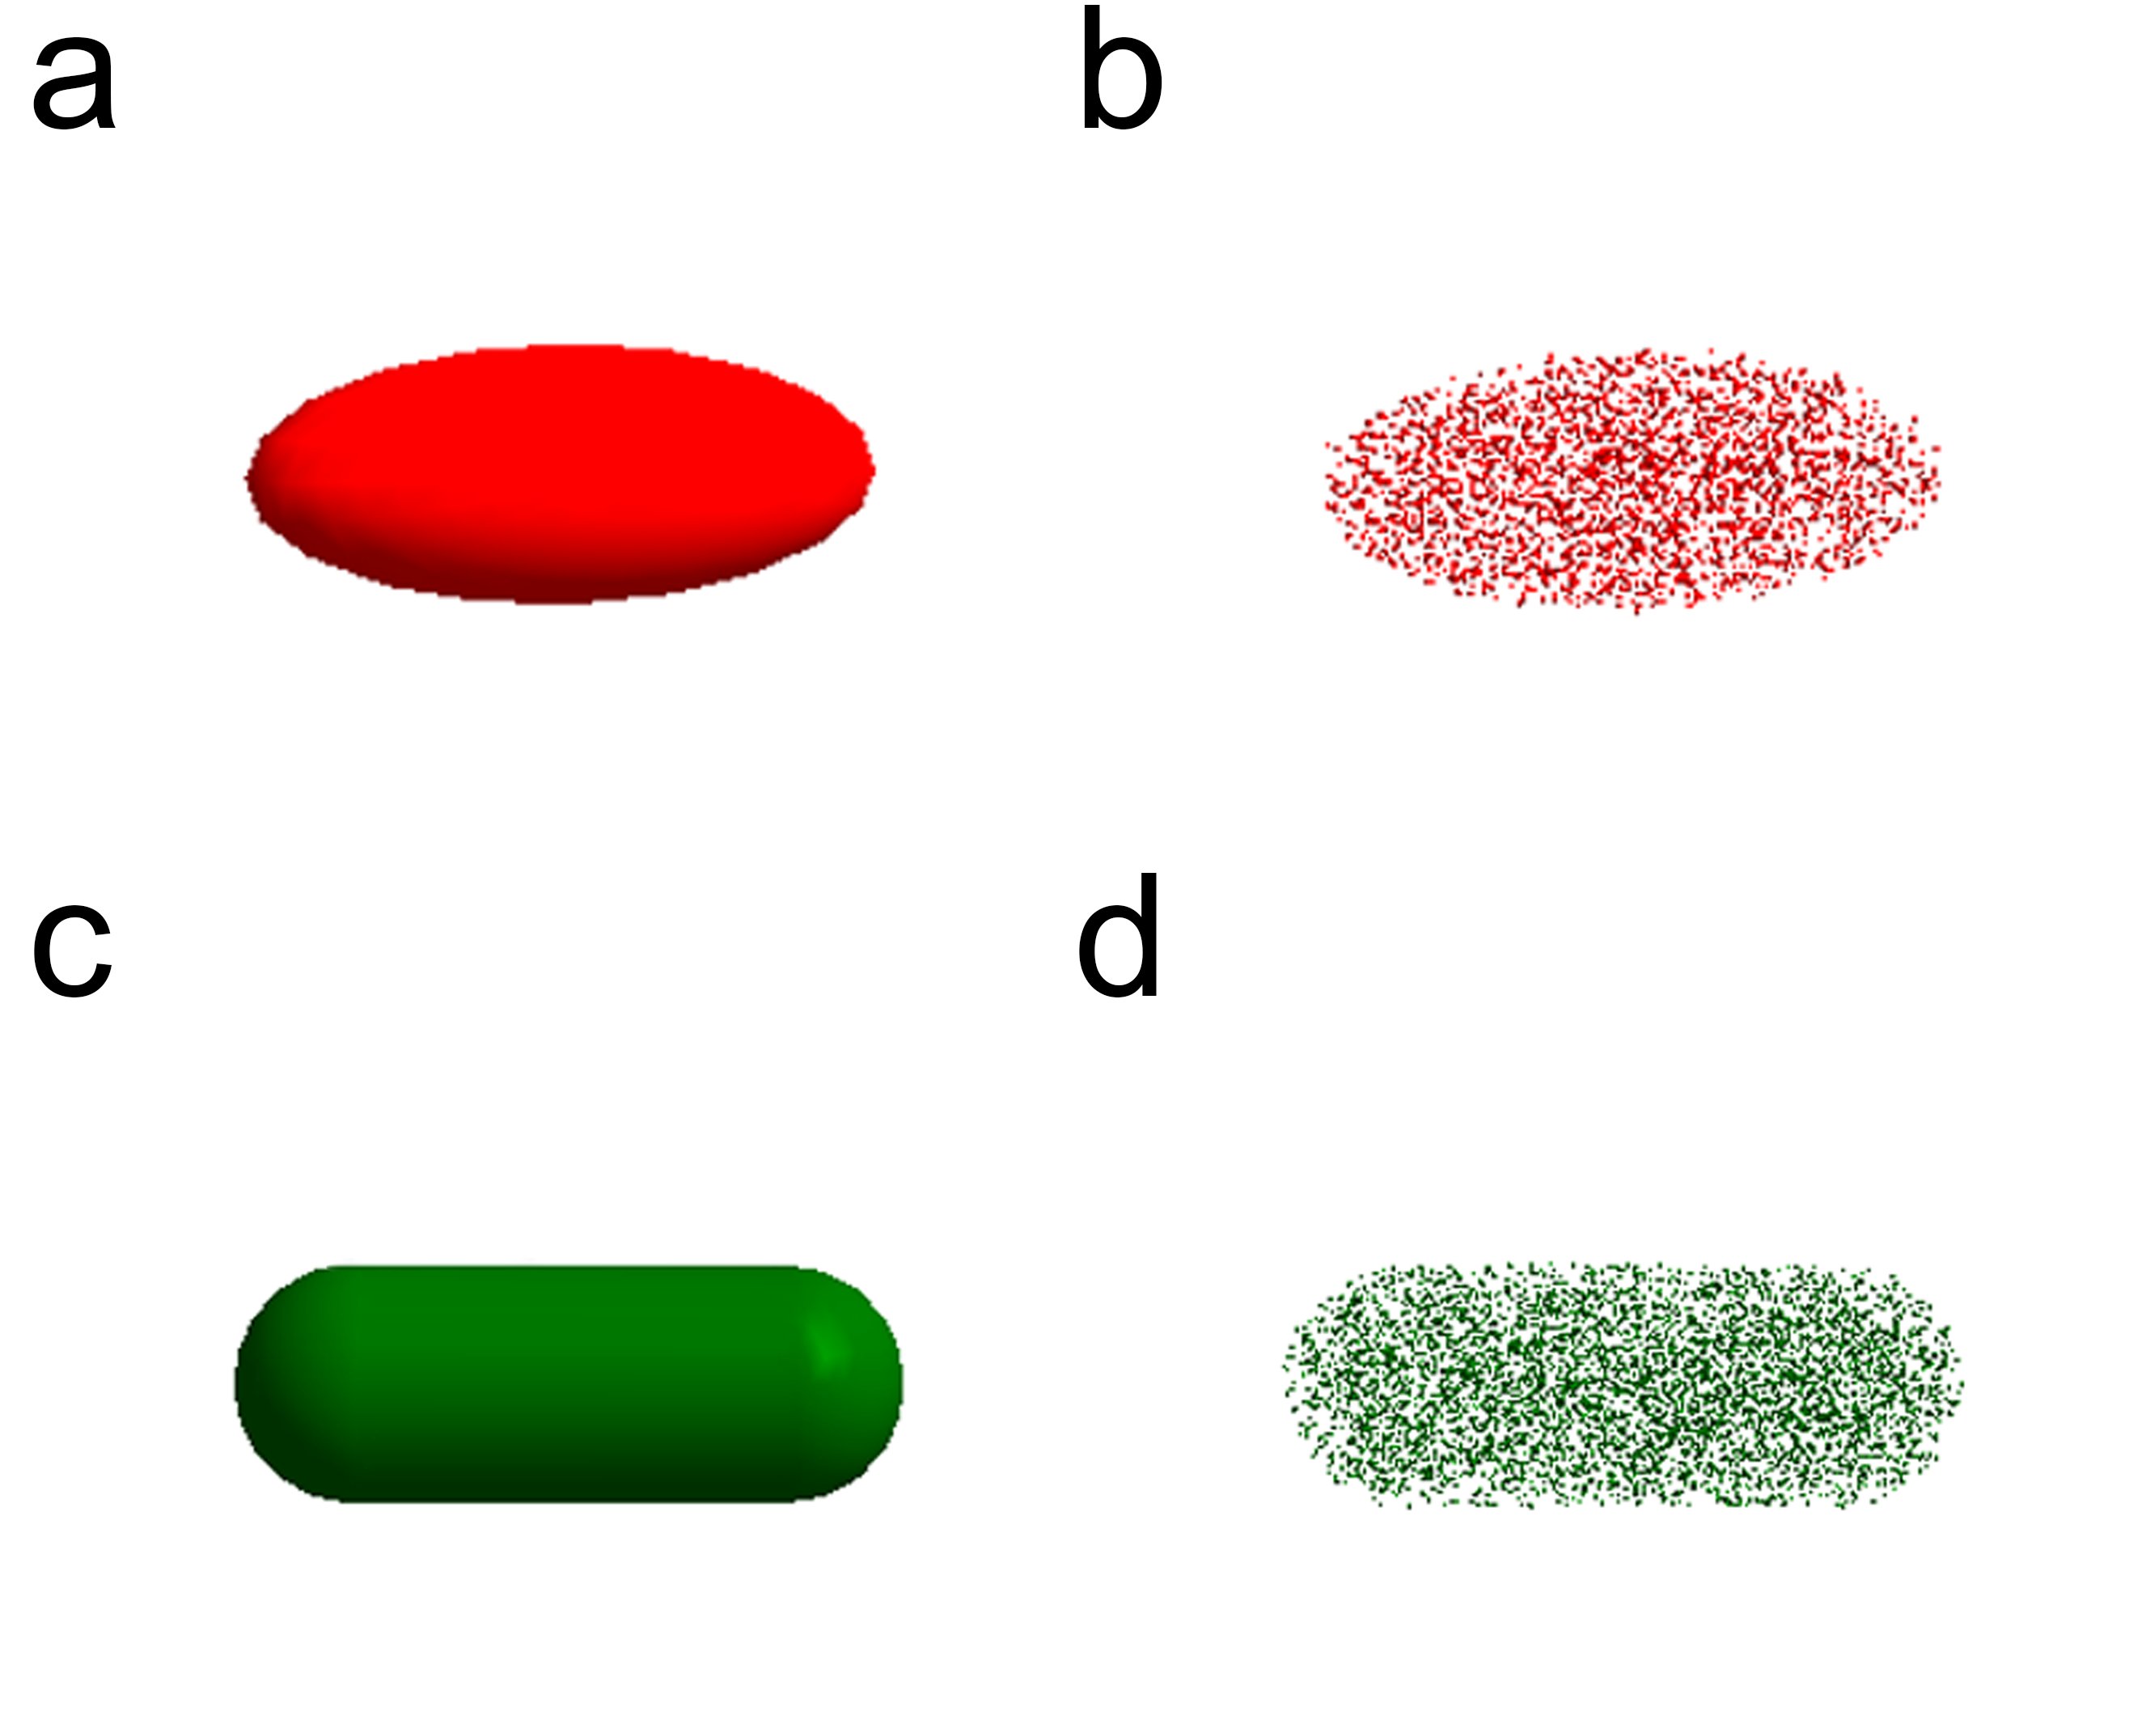
\includegraphics[width=0.5\columnwidth]{Scatteringmodel_single.png}
    \caption{Solid representations of a ellipsoid (a) and a spherocylinder (c). Mesh representations of a ellipsoid (b) and a spherocylinder (d).}
    \label{fig:scatt_mod_single}
\end{figure}

\begin{figure}
    \centering
    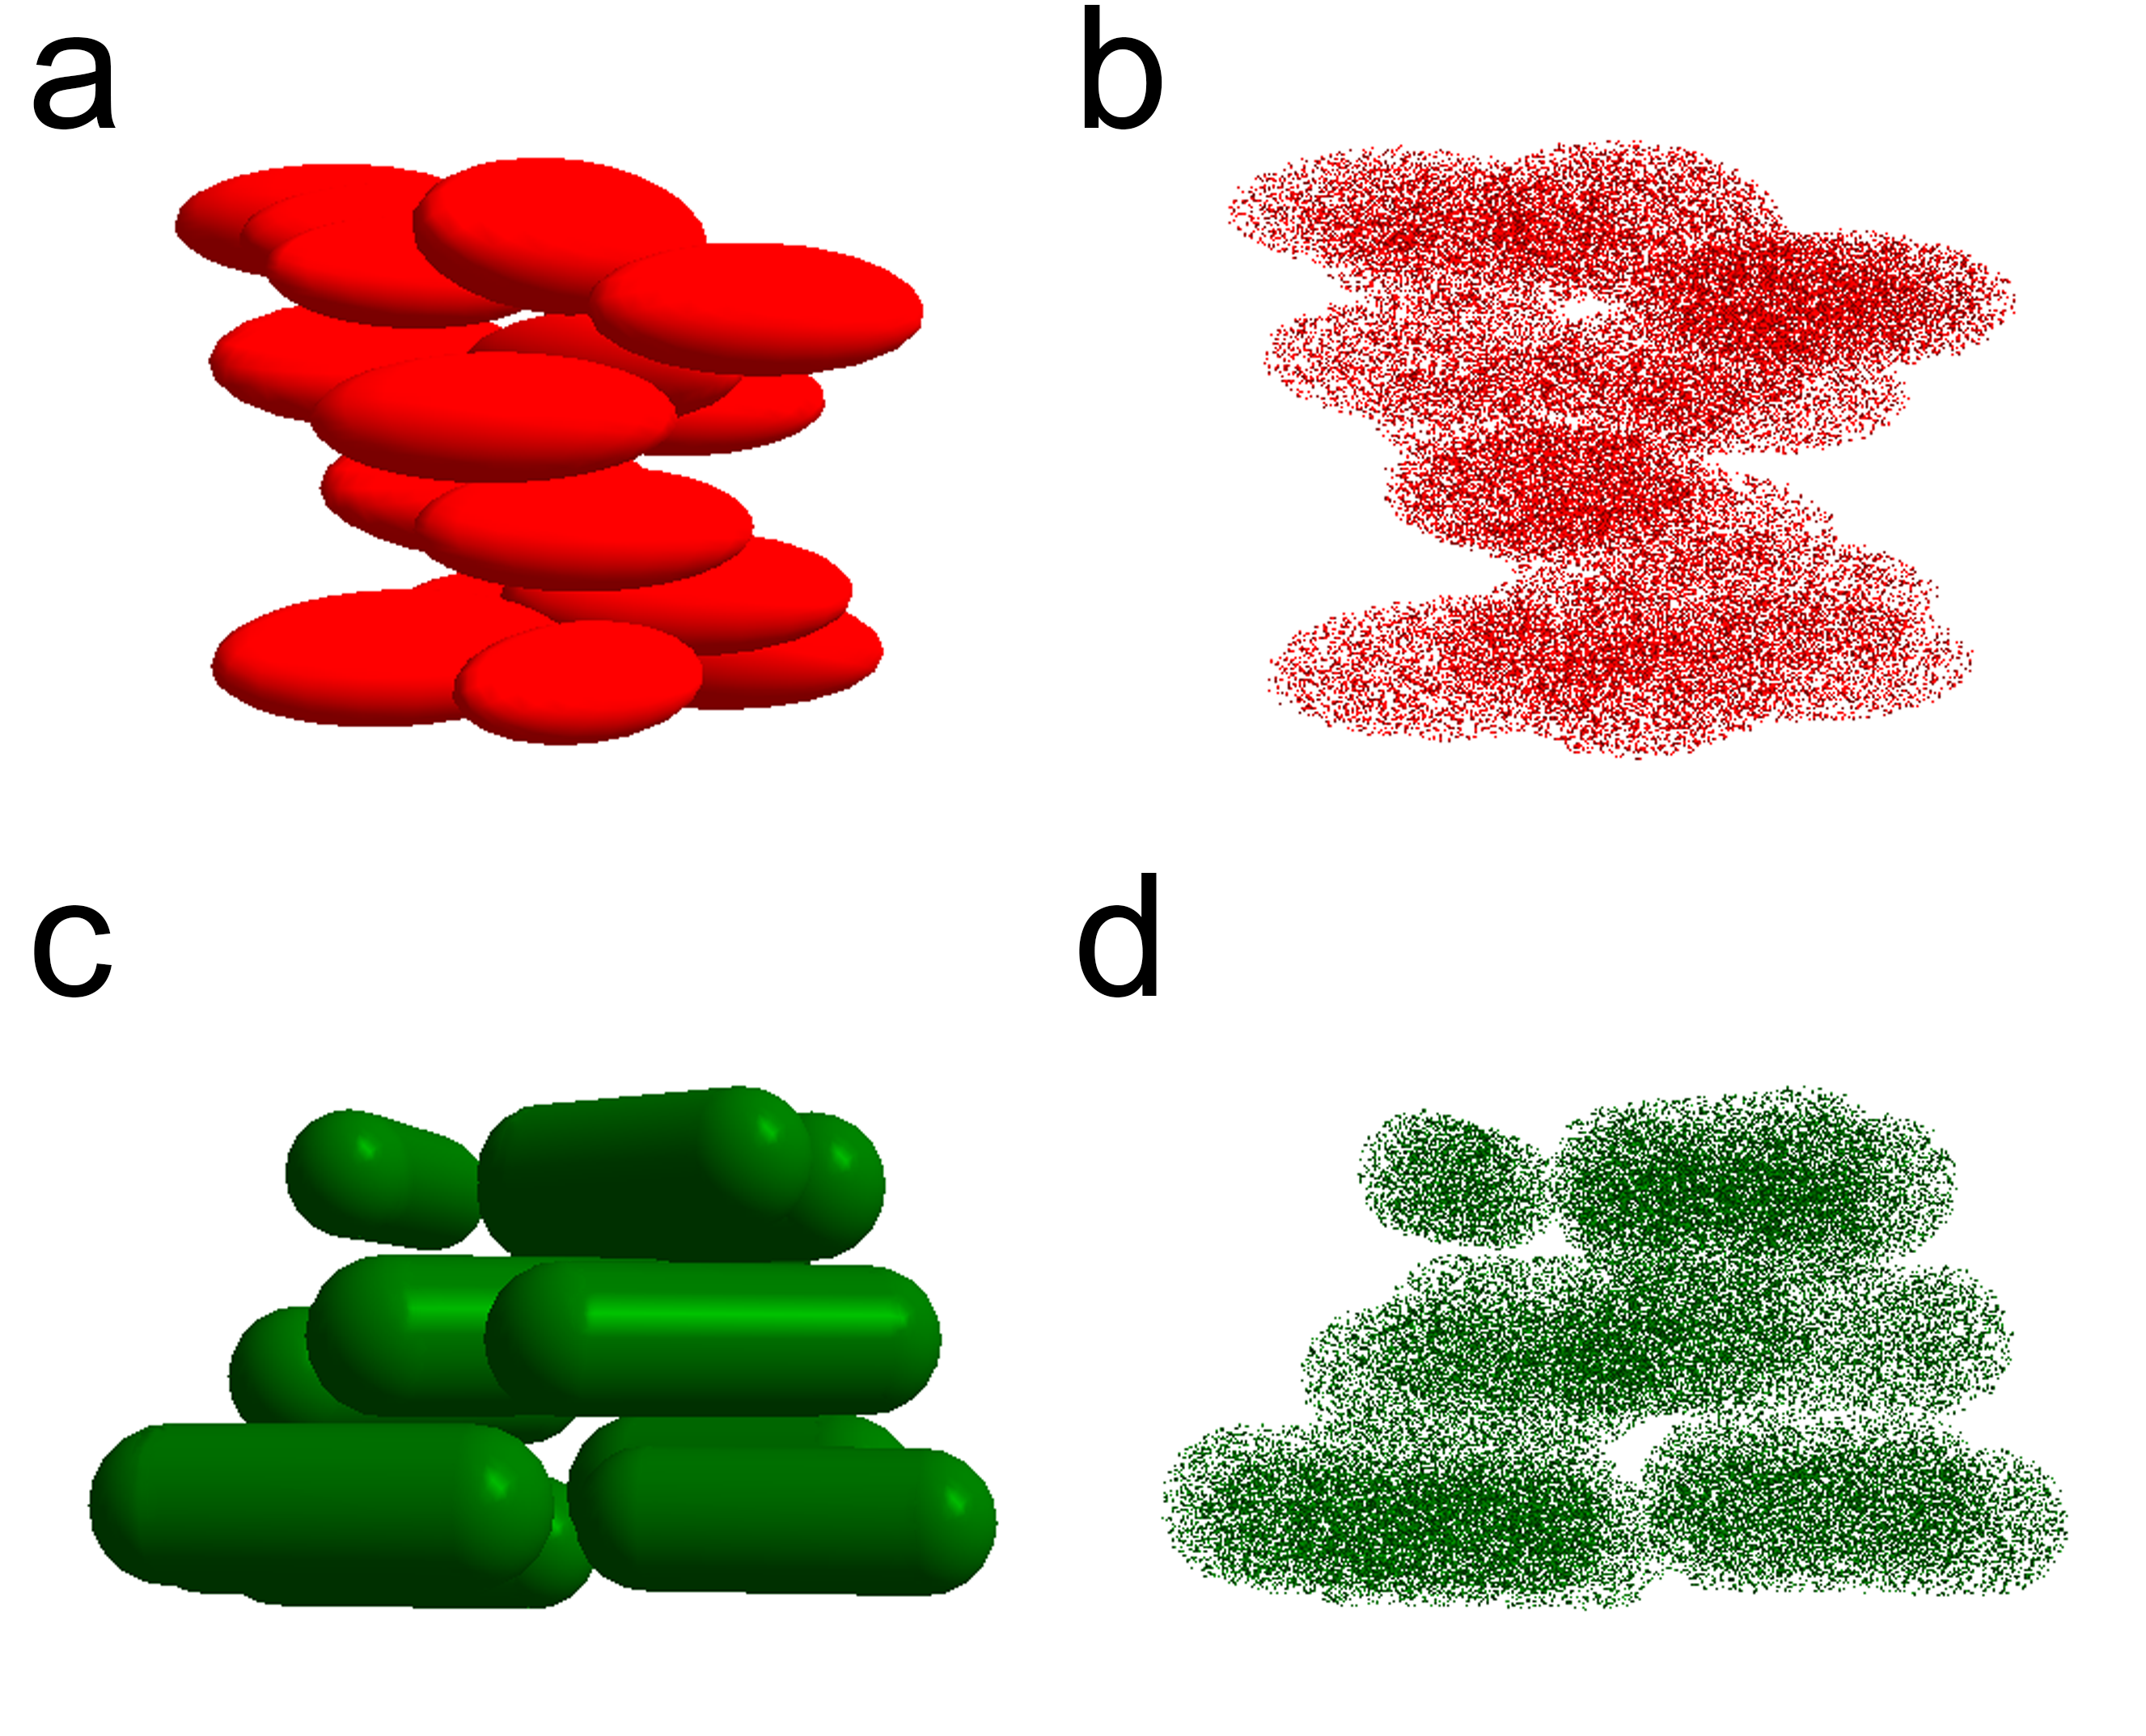
\includegraphics[width=0.5\columnwidth]{Scatteringmodel1.png}
    \caption{Example configurations for the structure factor calculation. Systems of ellipoids as solids (a) and meshes (b) and spherocylinders as solids (c) and meshes (d).}
    \label{fig:scatt_mod1}
\end{figure}

\begin{figure}
    \centering
    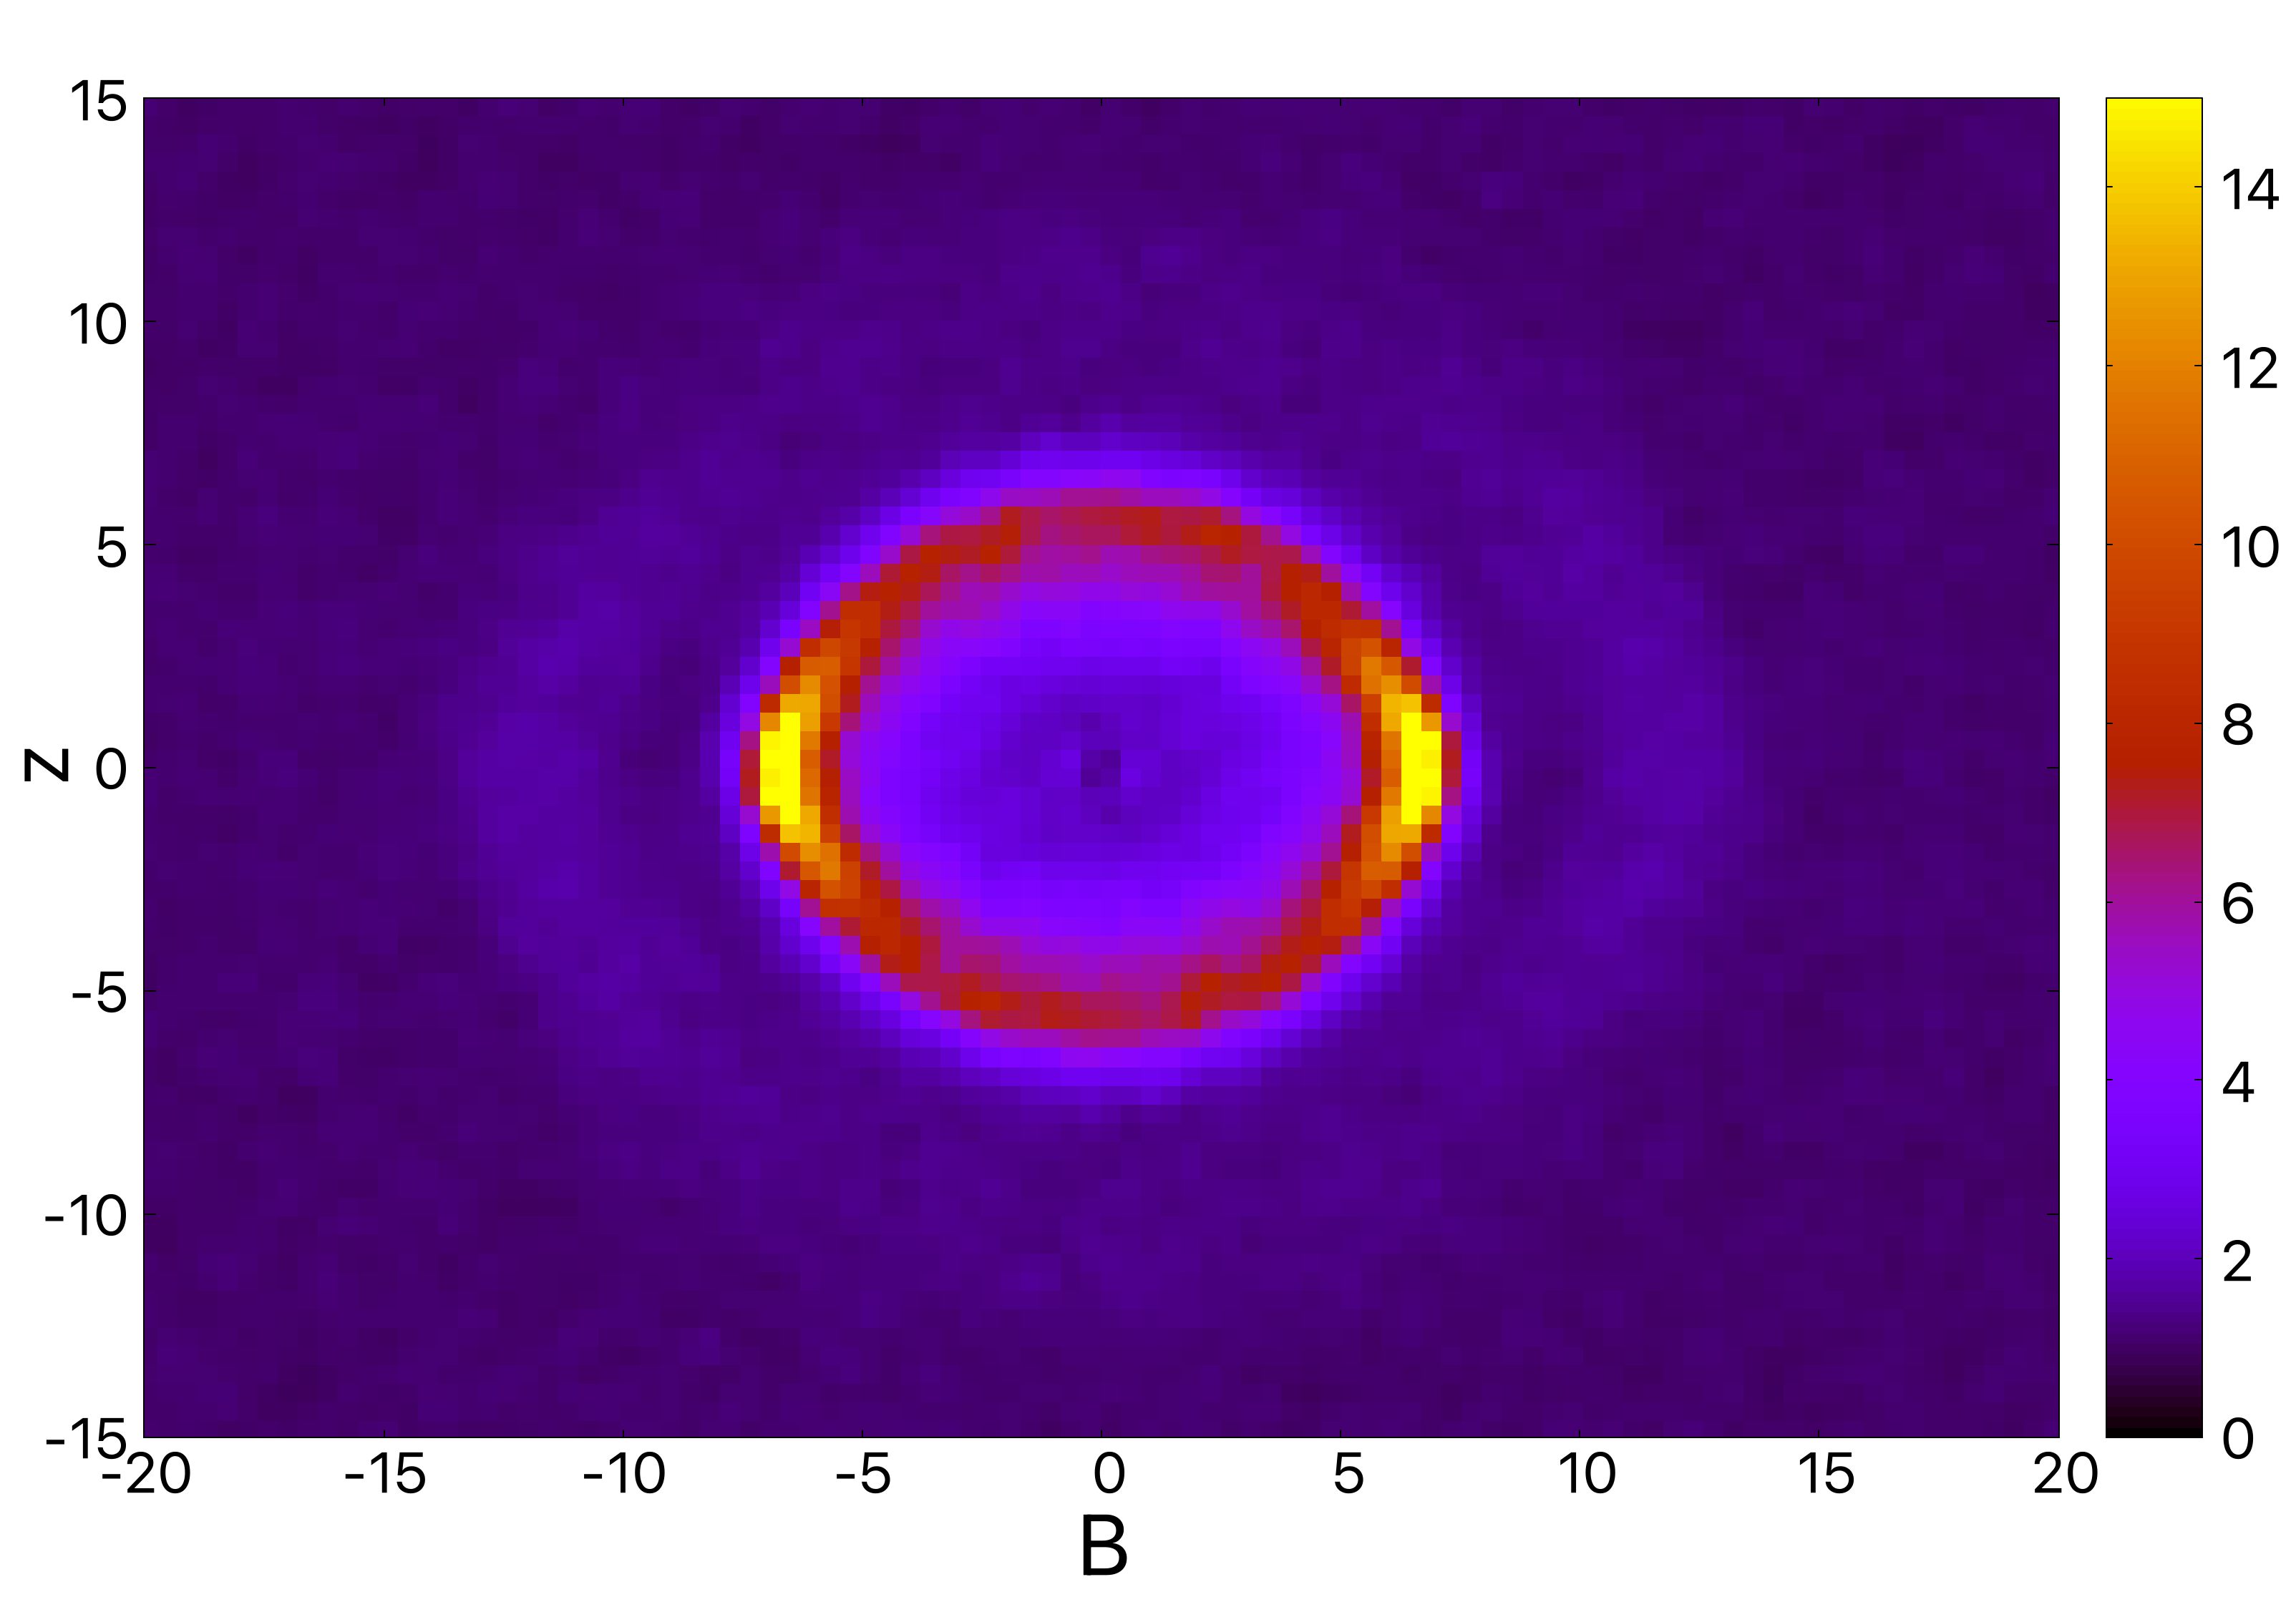
\includegraphics[width=1\columnwidth]{Syz_B_HE.png}
    \caption{Structure factor $S(0, q_y, q_z)$ of a system of spherocylinders with the presence of a magnetic field long the y axis at $\phi=0.50$.}
    \label{fig:Syz_B_HSC}
\end{figure}


\begin{figure}
    \centering
    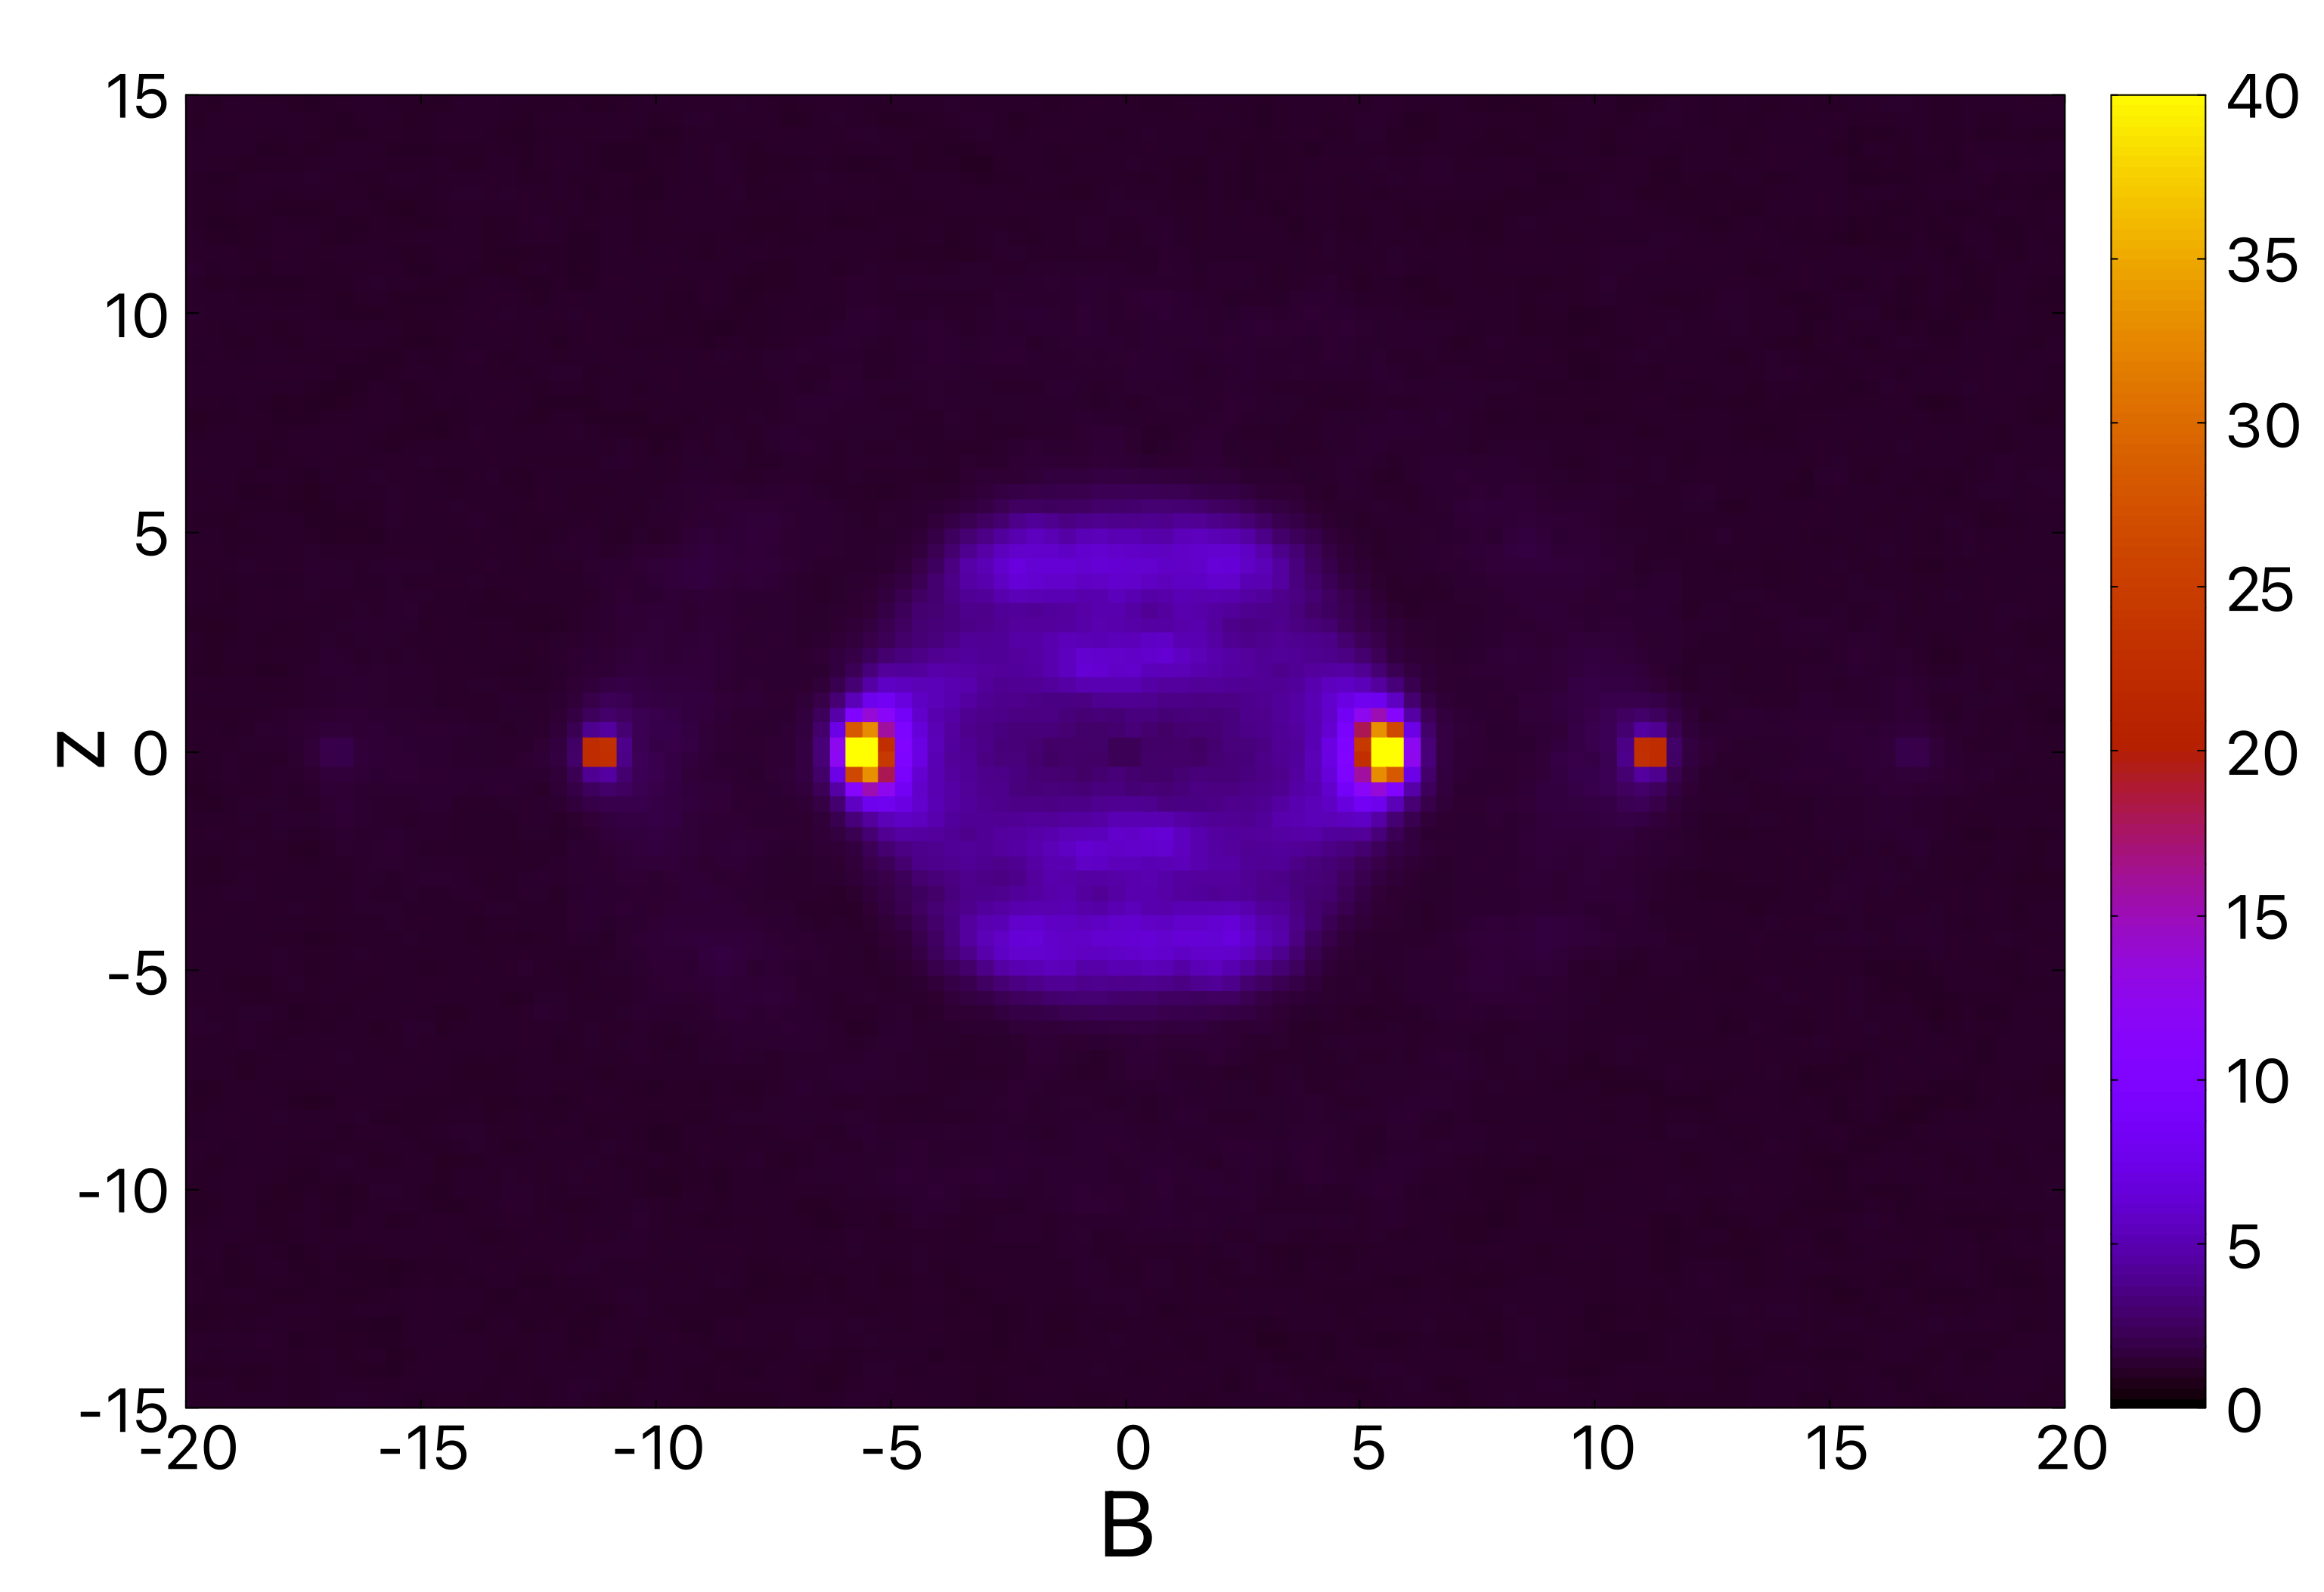
\includegraphics[width=1\columnwidth]{Syz_B.png}
    \caption{Structure factor $S(0, q_y, q_z)$ of a system of hard ellipsoids with the presence of a magnetic field long the y axis at $\phi=0.50$.}
    \label{fig:Syz_B_HE}
\end{figure}

\subsection{Pair distribution function}

The spatial characterization of the phases can be further analyzed by  the calculation of the three-dimensional pair distribution function $g(\vec{r})$:

\begin{equation}
    g(\vec{r}) = \frac{1}{\rho N} \left\langle \sum_{i=1}^N \sum_{j\neq i} \delta \left( \vec{r} - \left( \vec{r}_i - \vec{r}_j \right) \right) \right\rangle
\end{equation}

where $\delta(x)$ is the Dirac delta function. This quantity has been calculated averaging on the same configurations used for the structure factor \ref{eq:S_q}, obtaining the pair distribution function on a plane parallel to the magnetic field $yz$ and on the perpendicular plane $xz$. The results are represented in Fig. \ref{fig:gyz_B} and Fig. \ref{fig:gxz_B}. The smectic phase is evident: it can be noticed the different planes along the y axis (Fig. \ref{fig:gyz_B}) and the 2D liquid behaviour in-plane (Fig. \ref{fig:gxz_B}).
Differently the raddial distribution function of HEs does not show any layering for all state points studies.
A typical example of $g(r)$ for HEs is shown in Fig.\ref{fig:gyz_B_HE} (yz-plane) and Fig.~\ref{fig:gxz_B_HE} (xz-plane). 

\begin{figure}
    \begin{center}
    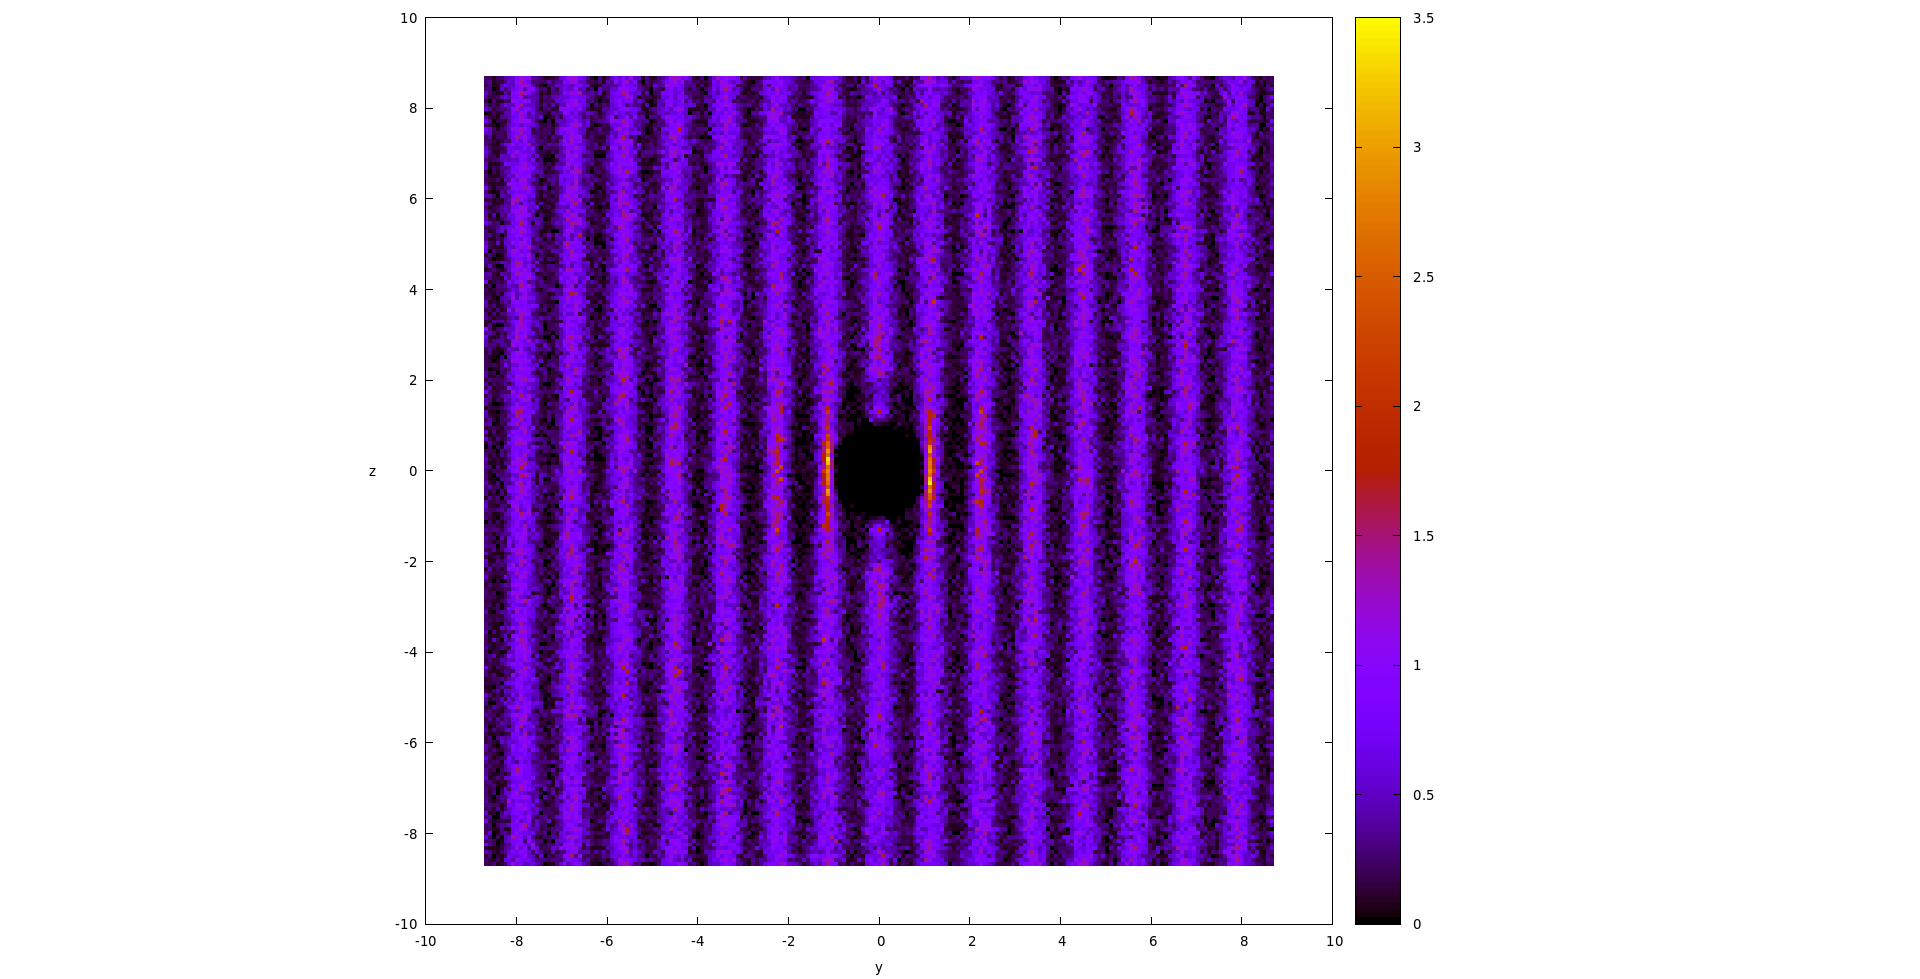
\includegraphics[width=1.0\columnwidth]{gyz_B.png}
    \caption{Pair distribution function for a system of spherocylinders $\phi = 0.50$ in presence of a magnetic field $\vec{B}$ along y axis.}
    \label{fig:gyz_B}
    \end{center}
\end{figure}


\begin{figure}
    \centering
    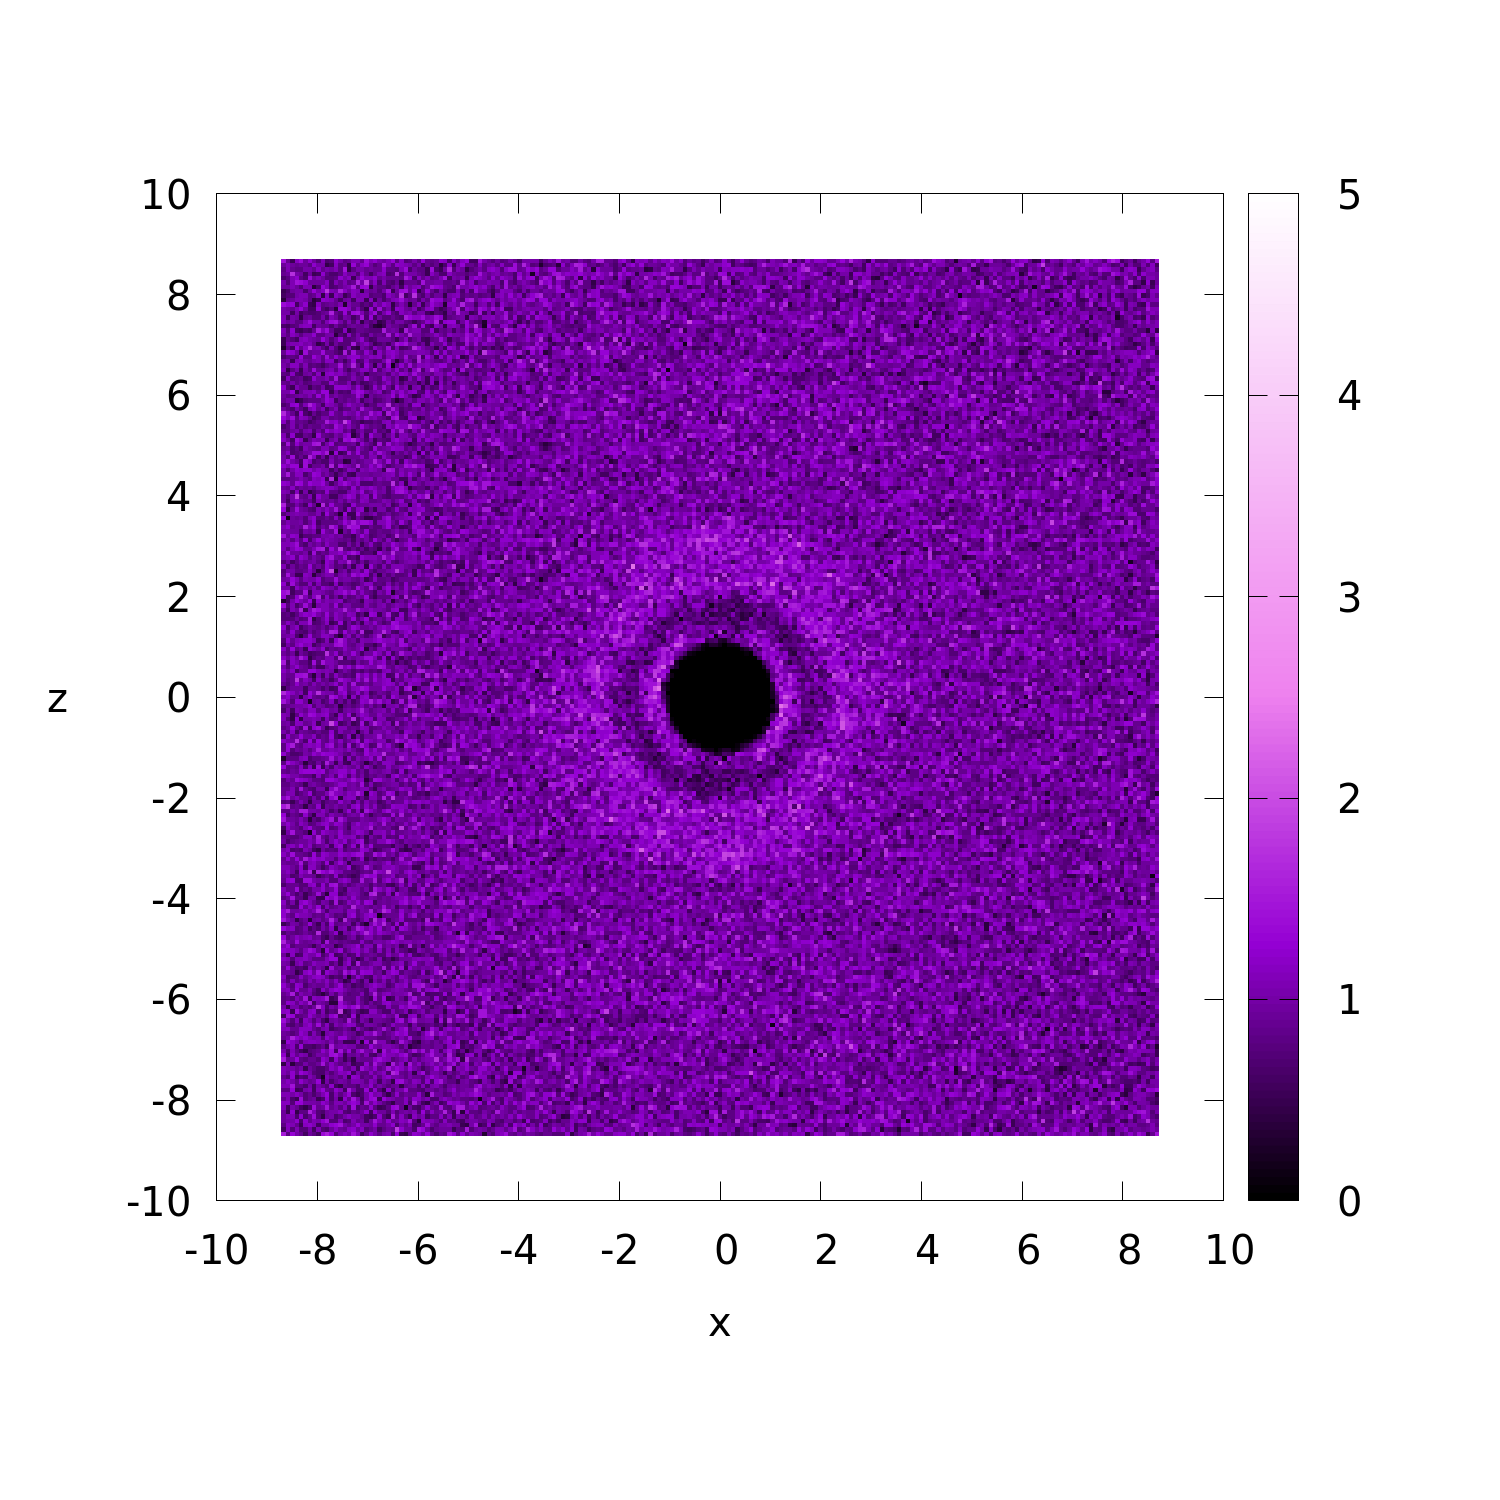
\includegraphics[width=1.0\columnwidth]{gxz_B.png}
    \caption{Pair distribution function for a system of spherocylinders $\phi = 0.50$ in presence of a magnetic field $\vec{B}$ along y axis.}
    \label{fig:gxz_B}
\end{figure}

\begin{figure}
    \begin{center}
    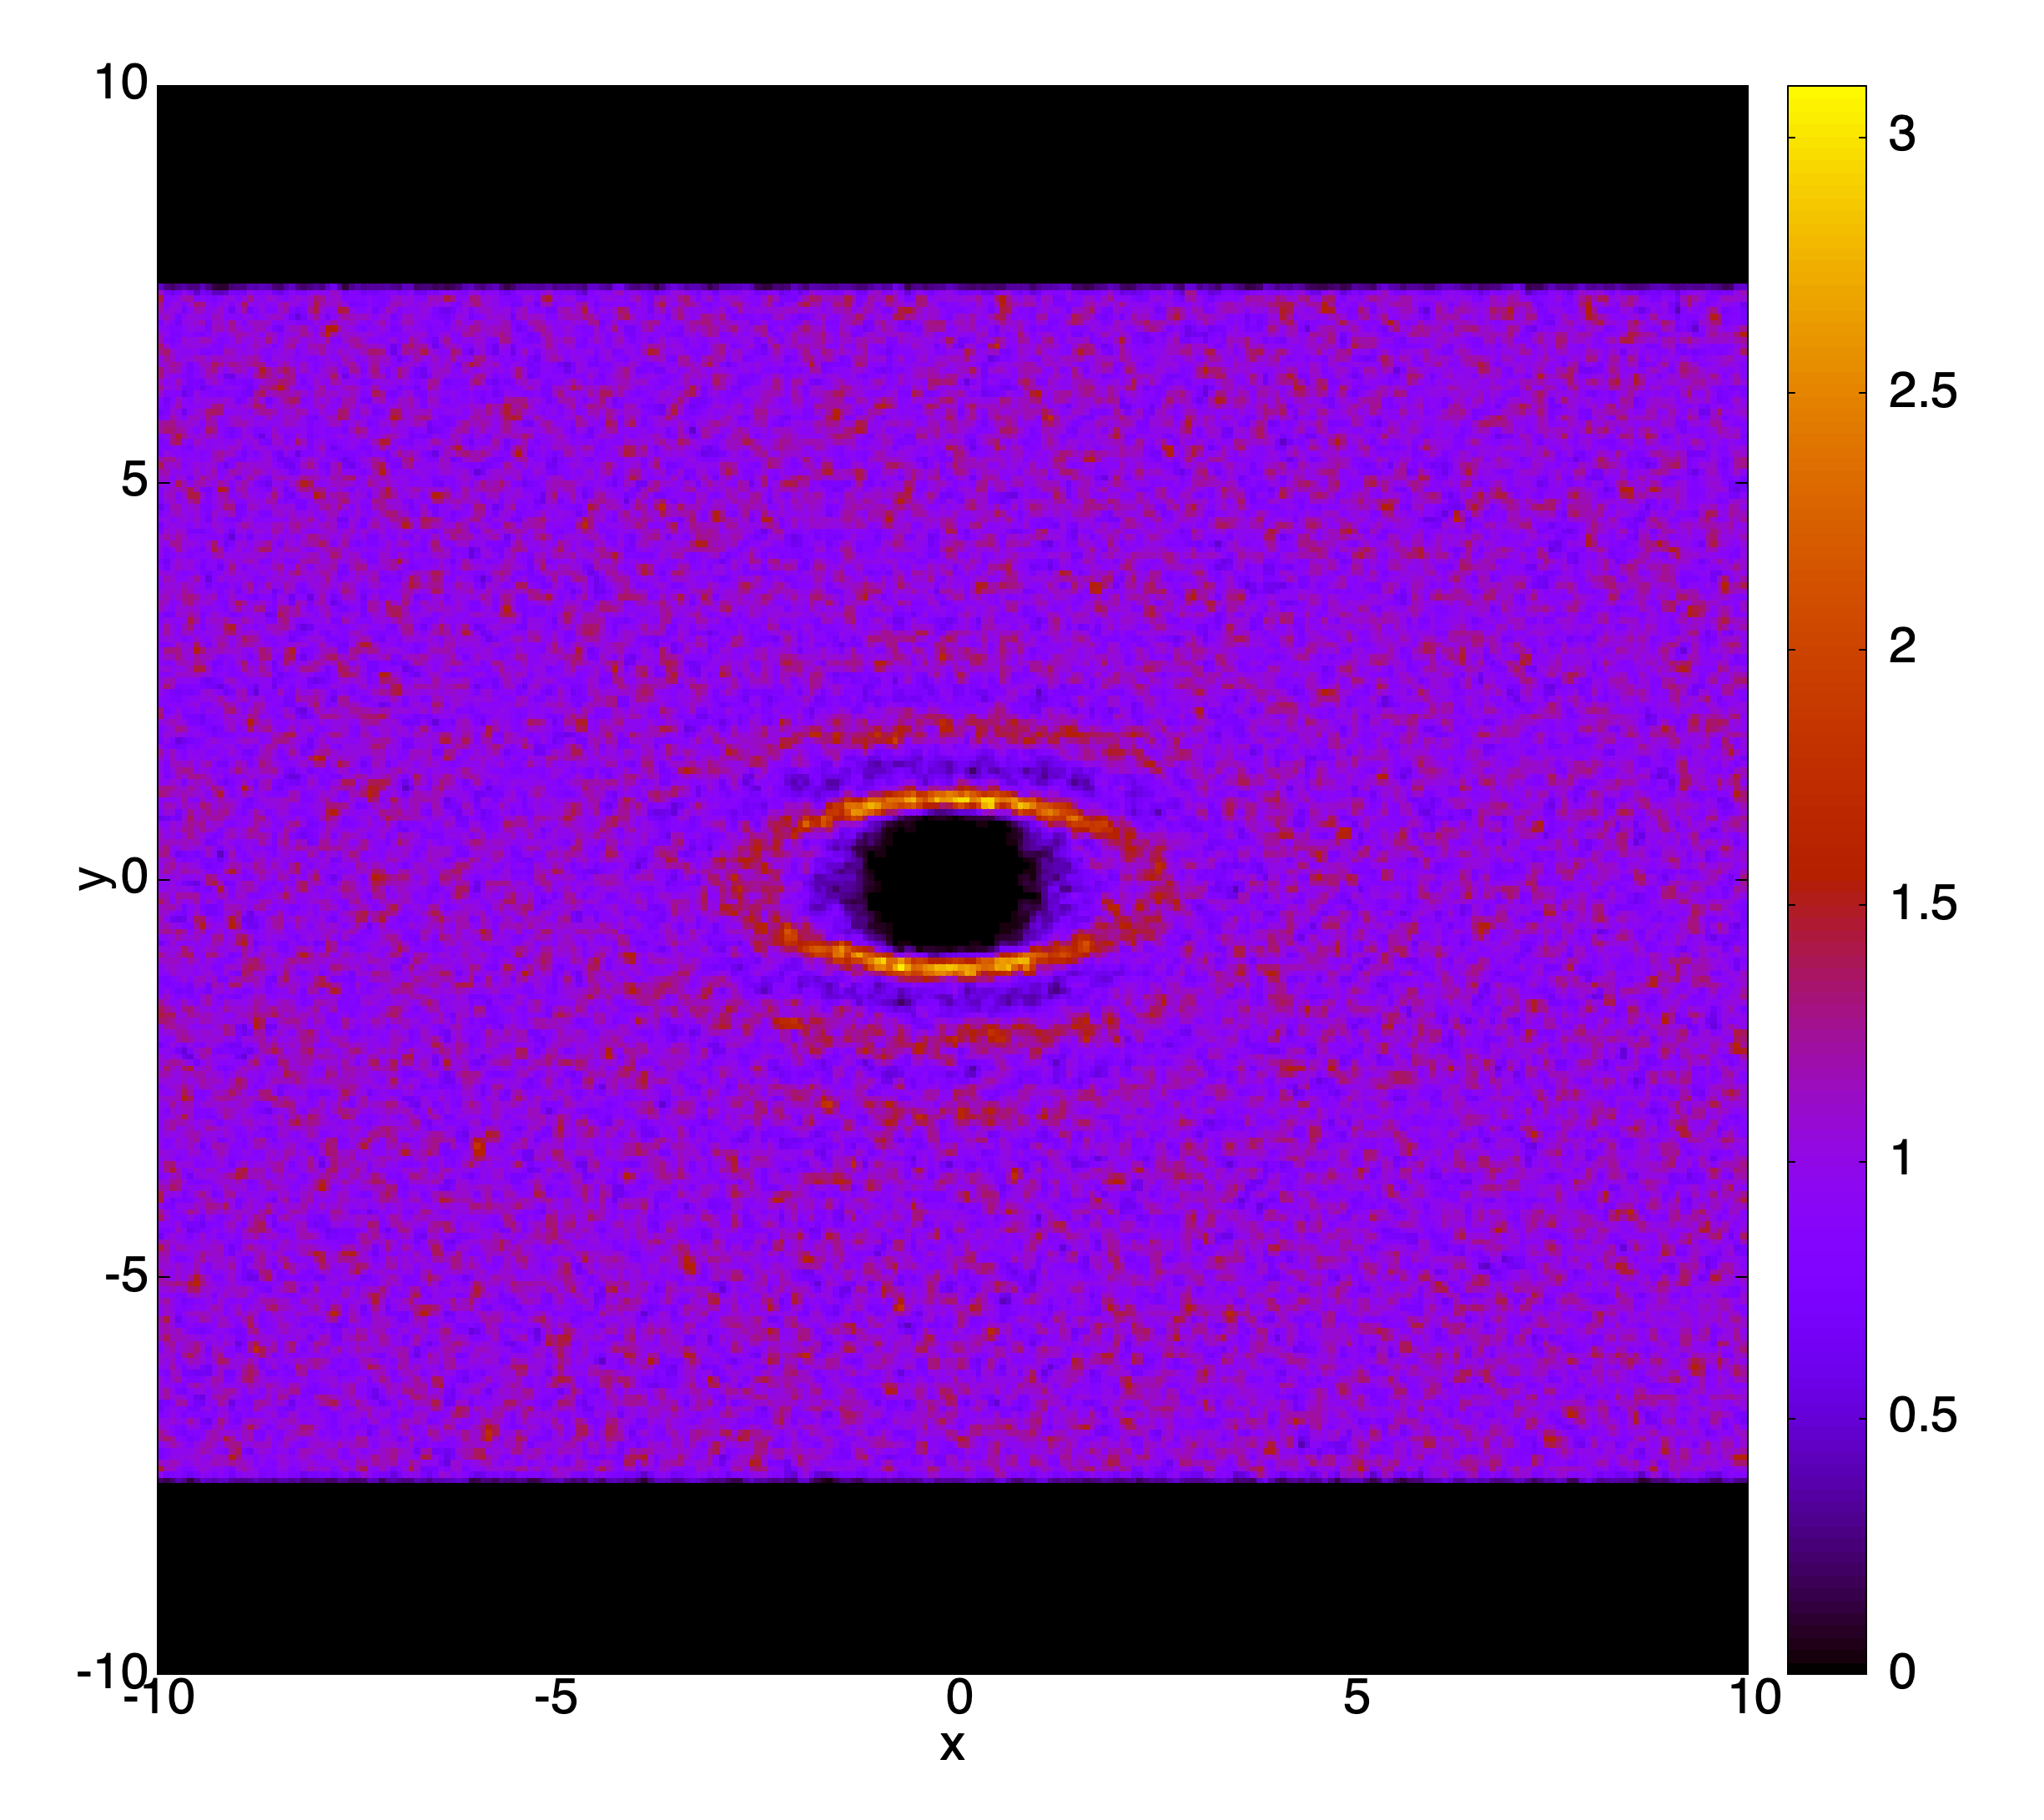
\includegraphics[width=1.0\columnwidth]{gyz_B_HE.png}
    \caption{Pair distribution function for a system of hard ellipsoids at $\phi = 0.50$ in presence of a magnetic field $\vec{B}$ along y axis.}
    \label{fig:gyz_B_HE}
    \end{center}
\end{figure}


\begin{figure}
    \centering
    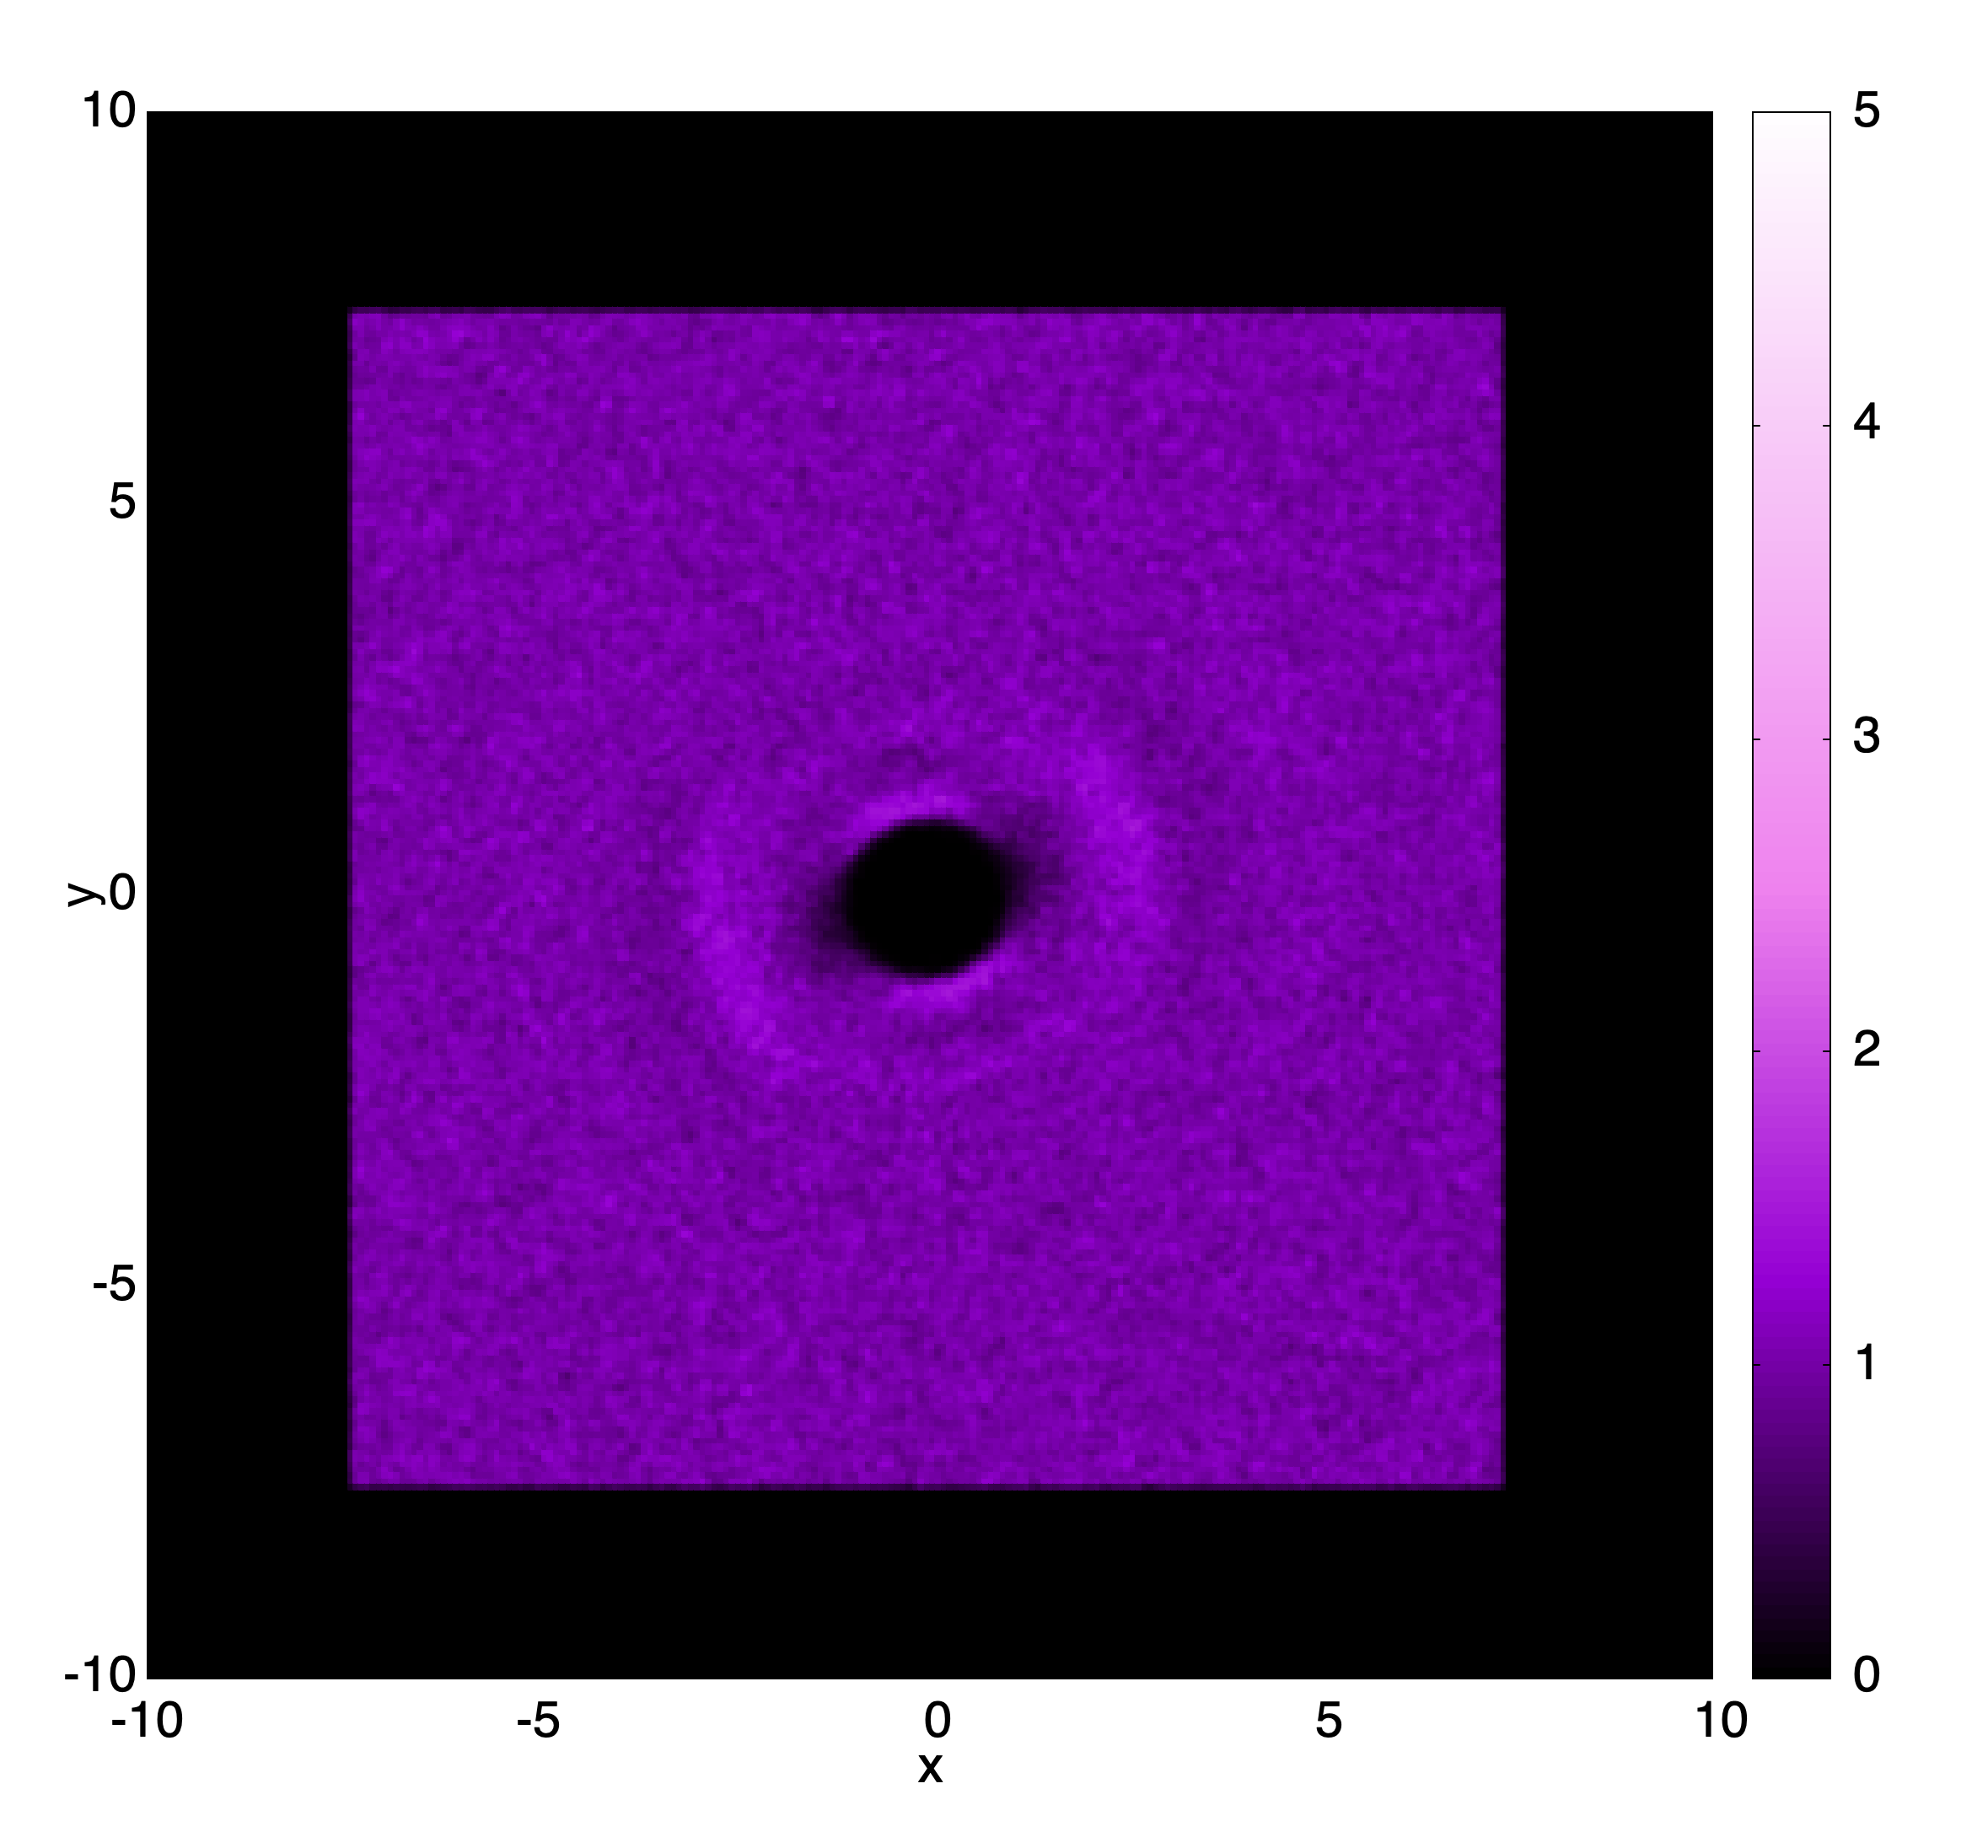
\includegraphics[width=1.0\columnwidth]{gxz_B_HE.png}
    \caption{Pair distribution function for a system of hard ellipsoids at $\phi = 0.50$ in presence of a magnetic field $\vec{B}$ along y axis.}
    \label{fig:gxz_B_HE}
\end{figure}
%\newpage %usato solo per non far andare l'immagine prima

\section{Absence of magnetic field}

In order to demonstrate the magnetic origin of the smectic phase in these systems, we performed a Monte Carlo simulation in the NVT ensemble of a smectic configuration of spherocylinders with $\phi = 0.50$. As represented in Fig. \ref{fig:noB_snapshot}, in absence of a magnetic field the system preferentially arranges in a isotropic phase.

\subsection{Structure factor}
To further confirm the isotropy of this phase, it has been calculated the structure factor $S(0, q_y, q_z)$ of the system which presents a typical isotropic pattern (Fig. \ref{fig:Syz_noB}).

%\newpage    %da togliere

\begin{figure}
    \centering
    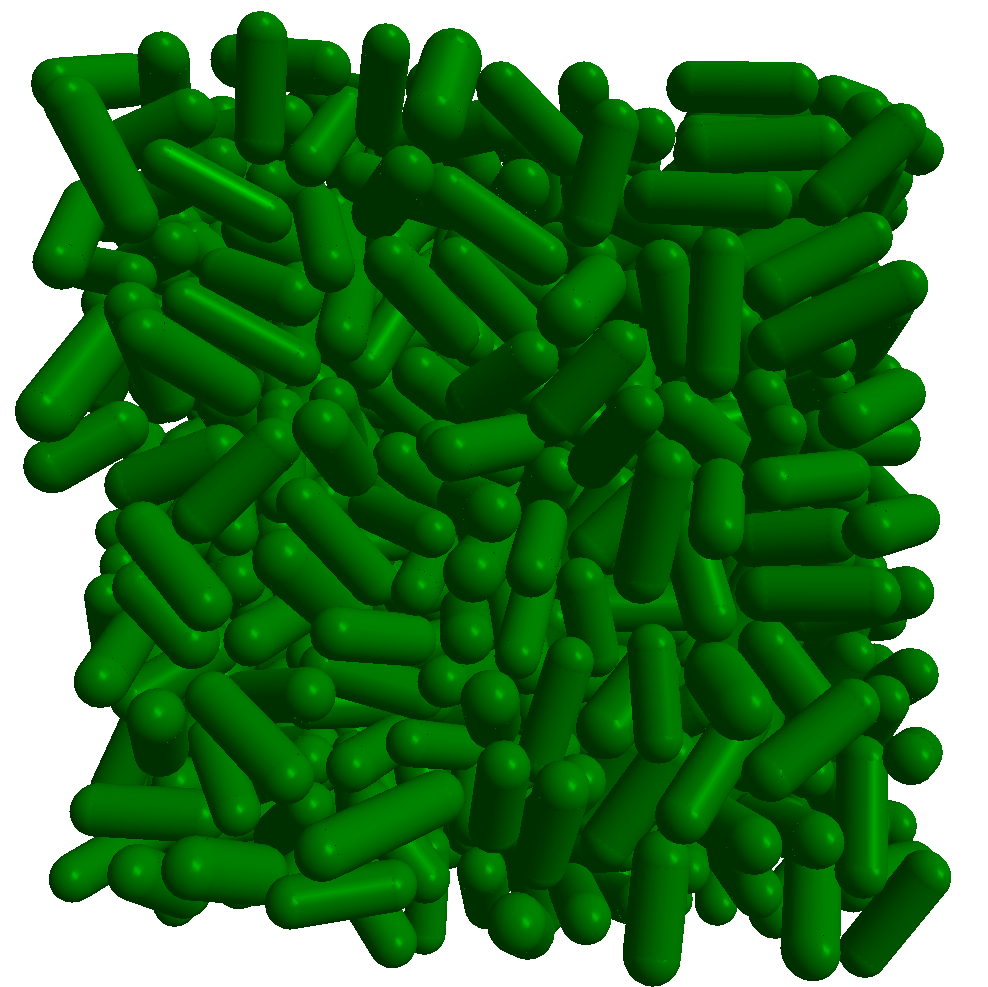
\includegraphics[width=0.5\columnwidth]{Isotropic_phase_snap.png}
    \caption{Snapshot of a system of polydisperse spherocylinders with $\phi = 0.50$ in absence of magnetic field.}
    \label{fig:noB_snapshot}
\end{figure}

\begin{figure}
    \centering
    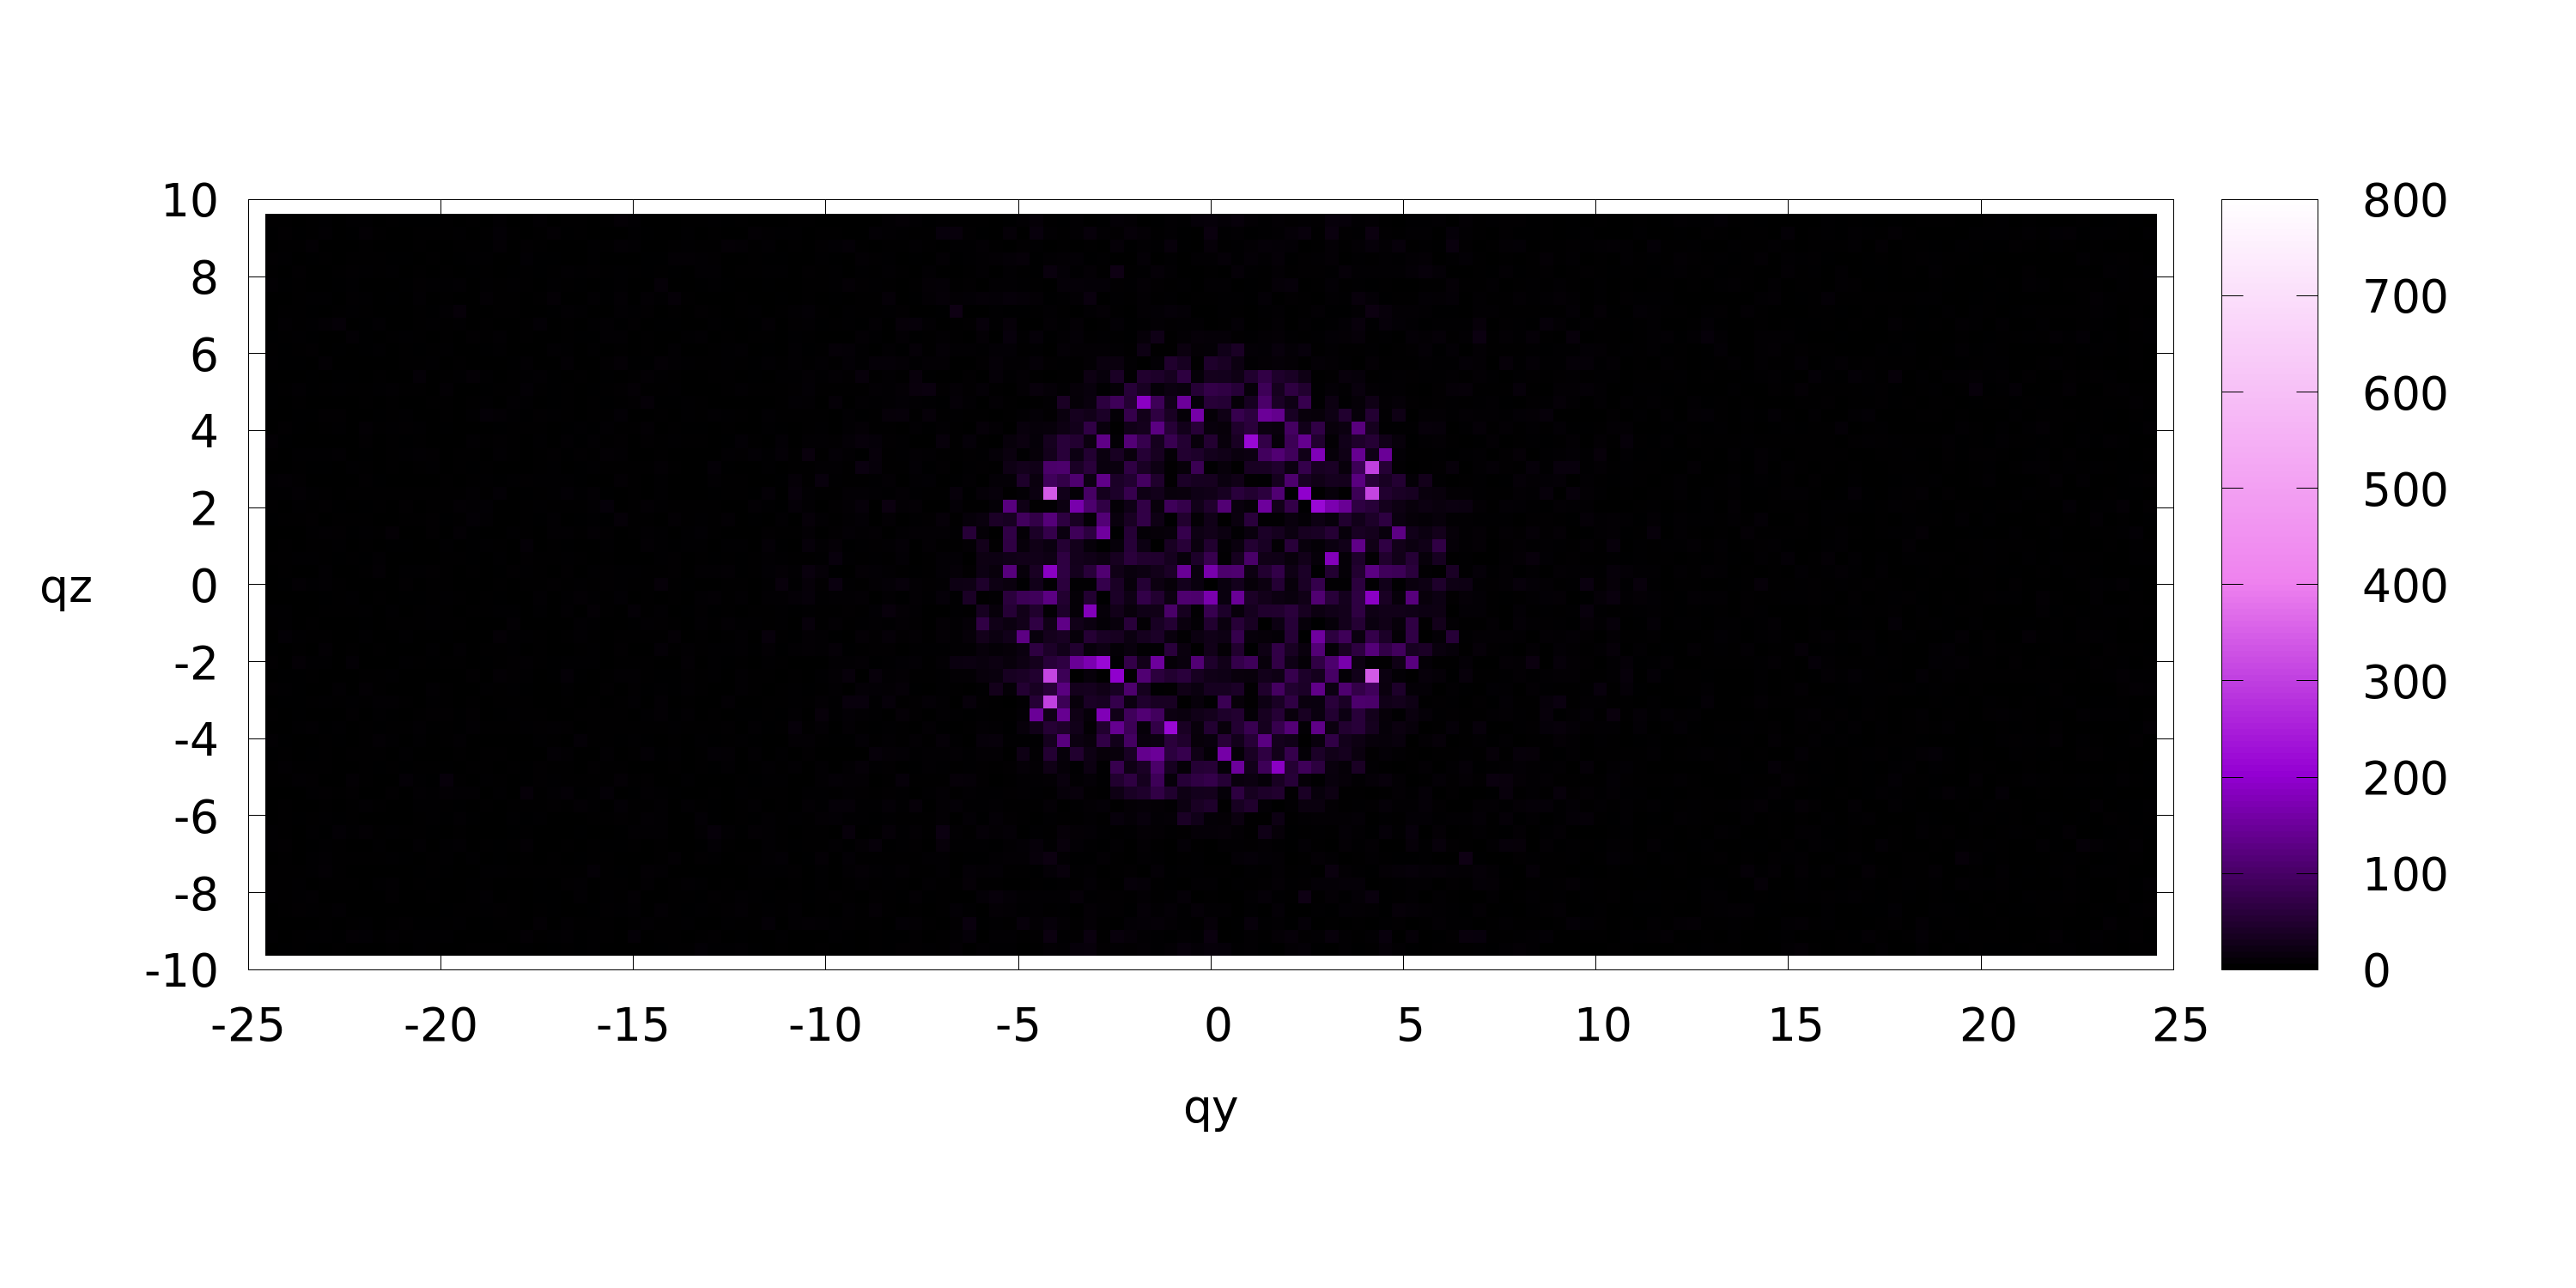
\includegraphics[width=1\columnwidth]{Syz_noB.png}
    \caption{Structure factor $S(0, q_y, q_z)$ of the system in absence of magnetic field.}
    \label{fig:Syz_noB}
\end{figure}


\subsection{Pair distribution function}

Likewise the case with a magnetic field, it has been calculated the pair distribution function of a system of spherocylinders in absence of magnetic field. As it can be seen from Fig. \ref{fig:gxz_noB} and Fig. \ref{fig:gyz_noB}, the phase is clearly isotropic, without long range spatial correlation between the particles, corroborating the magnetic field induced nature of the smectic phase.


\begin{figure}
    \centering
    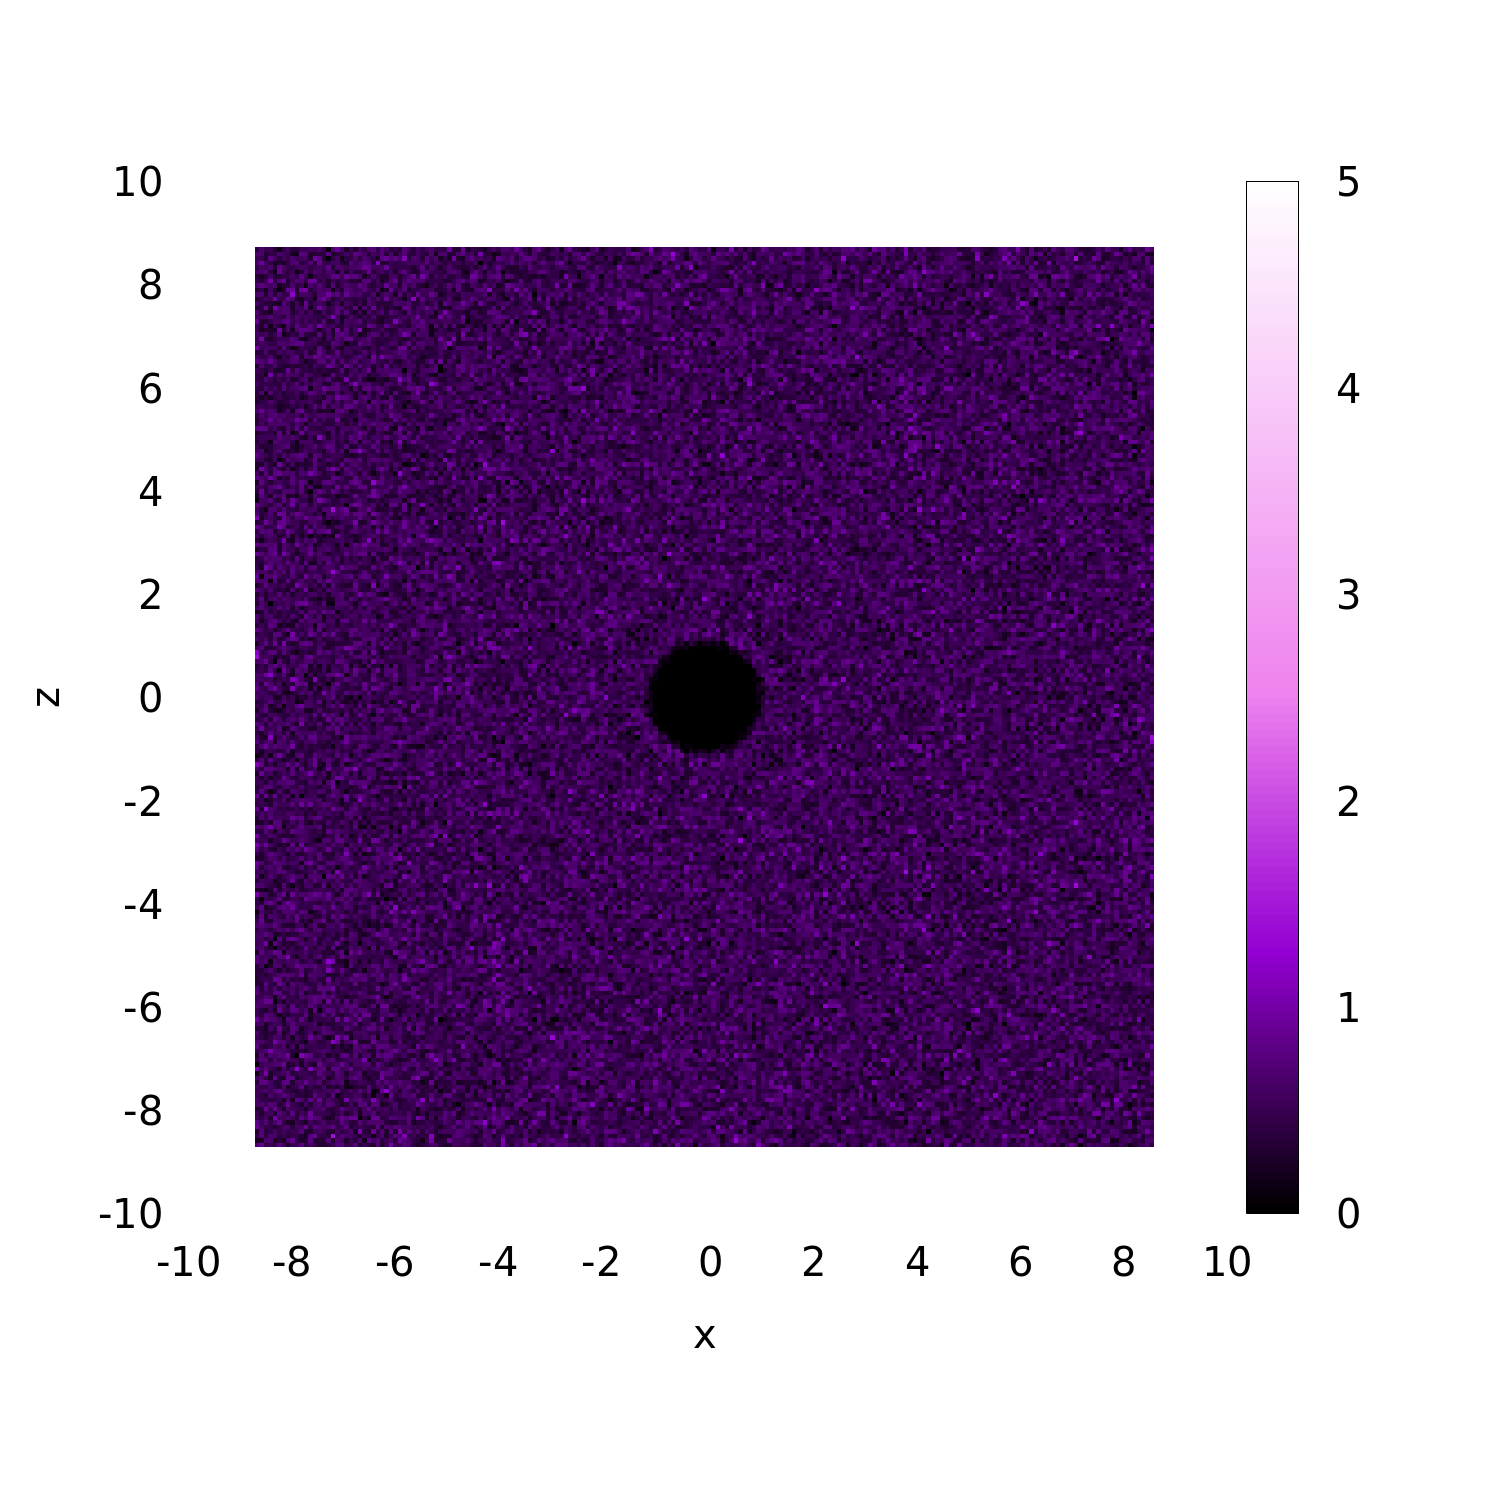
\includegraphics[width=1\columnwidth]{gxz_noB.png}
    \caption{Pair distribution function of the system on the xz-plane without a magnetic field.}
    \label{fig:gxz_noB}
\end{figure}


\begin{figure}
    \centering
    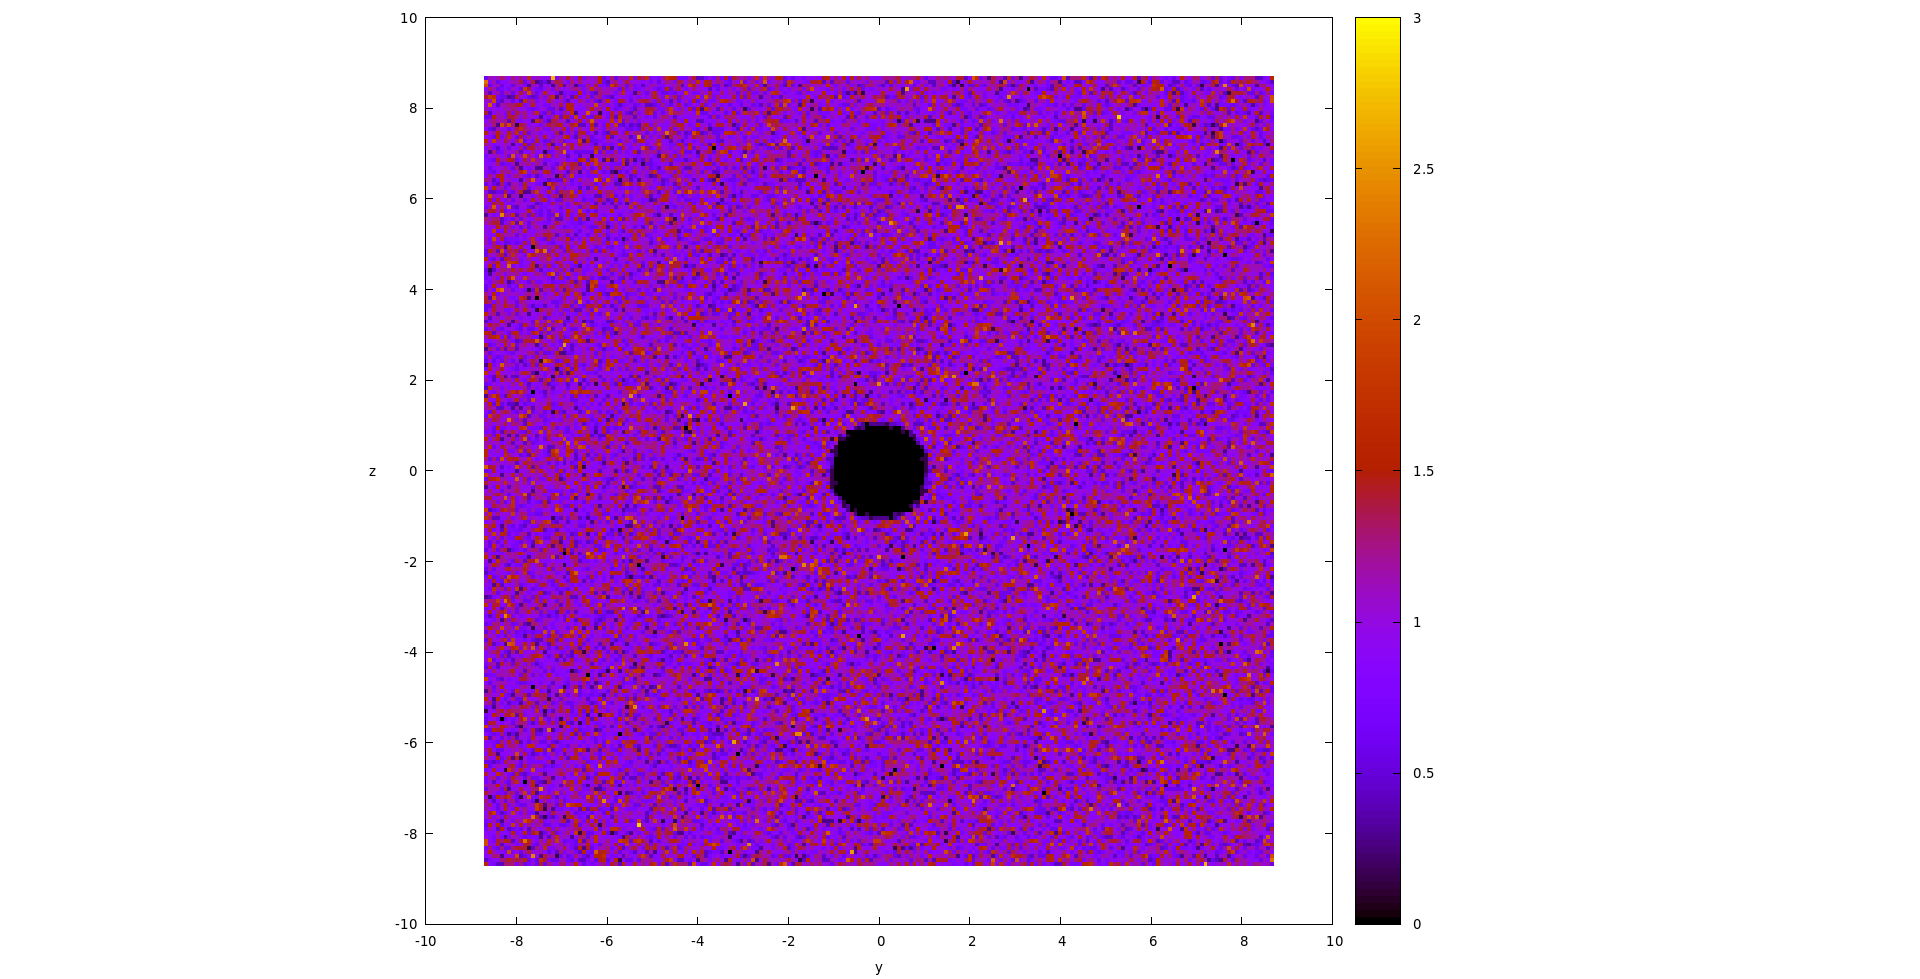
\includegraphics[width=1\columnwidth]{gyz_noB.png}
    \caption{Pair distribution function of the system on the yz-plane without a magnetic field.}
    \label{fig:gyz_noB}
\end{figure}

\newpage

\section{Smectic order parameter}

A convenient way to check for the emergence of a smectic phase in our computer simulations 
is to calculate the smectic order parameter $\tau_1$ defined as follows:

\begin{equation}
    \tau_1 = \langle | \sum_i e^{i 2\pi \vec{r}_i \cdot \hat{n} / d } |\rangle 
\end{equation}

where $\langle\ldots\rangle$ is an average over several independent configurations, $\vec{r}_i$ is the position of the $i$-th particle, $\hat{n}$ is the direction of the magnetic
field and $d$ is the thickness of the smectic layers.
In order to compute $\tau_1$ for each configuration we find the optimal value of $d$, i.e. 
the value which maximizes $\tau_1$.

The values of $\tau_1$ for both HSCs and HEs and for all pressures studied is shown in Fig.~\ref{fig:smordpar}. It can be seen that HSCs exhibit a range of volume fractions where 
a smectic layer ordering is present and which coincide with the green state points shown in Fig. 7(a)
in the main test. On the contrary no evidence of layering emerges in the simulation of HEs.

\begin{figure}
    \centering
    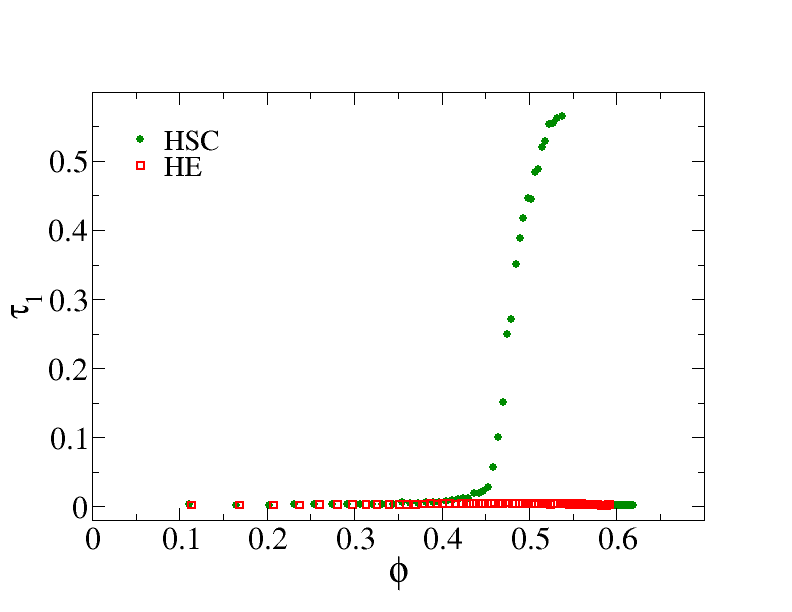
\includegraphics[width=1\columnwidth]{smordpar.png}
    \caption{Smectic order parameter $\tau_1$ for HSCs and HEs.}
    \label{fig:smordpar}
\end{figure}

\begin{thebibliography}{1}
\bibitem{Hansen_McDonald}
Jean-Pierre Hansen, Ian R. McDonald.
\newblock Theory of Simple Liquids (Fourth Edition), With Applications to Soft Matter.
\newblock In {\em Academic Press}, 2013. ISBN: 978-0-12-387032-2


\end{thebibliography}

\end{document}
